\documentclass[ignorenonframetext,]{beamer}
\setbeamertemplate{caption}[numbered]
\setbeamertemplate{caption label separator}{: }
\setbeamercolor{caption name}{fg=normal text.fg}
\beamertemplatenavigationsymbolsempty
\usepackage{lmodern}
\usepackage{amssymb,amsmath}
\usepackage{ifxetex,ifluatex}
\usepackage{fixltx2e} % provides \textsubscript
\ifnum 0\ifxetex 1\fi\ifluatex 1\fi=0 % if pdftex
  \usepackage[T1]{fontenc}
  \usepackage[utf8]{inputenc}
\else % if luatex or xelatex
  \ifxetex
    \usepackage{mathspec}
  \else
    \usepackage{fontspec}
  \fi
  \defaultfontfeatures{Ligatures=TeX,Scale=MatchLowercase}
\fi
\usetheme[]{CambridgeUS}
\usecolortheme{beaver}
\usefonttheme{structurebold}
% use upquote if available, for straight quotes in verbatim environments
\IfFileExists{upquote.sty}{\usepackage{upquote}}{}
% use microtype if available
\IfFileExists{microtype.sty}{%
\usepackage{microtype}
\UseMicrotypeSet[protrusion]{basicmath} % disable protrusion for tt fonts
}{}
\newif\ifbibliography
\hypersetup{
            pdftitle={Geodaten - zweiter Teil},
            pdfauthor={Jan-Philipp Kolb},
            pdfborder={0 0 0},
            breaklinks=true}
\urlstyle{same}  % don't use monospace font for urls
\usepackage{color}
\usepackage{fancyvrb}
\newcommand{\VerbBar}{|}
\newcommand{\VERB}{\Verb[commandchars=\\\{\}]}
\DefineVerbatimEnvironment{Highlighting}{Verbatim}{commandchars=\\\{\}}
% Add ',fontsize=\small' for more characters per line
\usepackage{framed}
\definecolor{shadecolor}{RGB}{248,248,248}
\newenvironment{Shaded}{\begin{snugshade}}{\end{snugshade}}
\newcommand{\KeywordTok}[1]{\textcolor[rgb]{0.13,0.29,0.53}{\textbf{#1}}}
\newcommand{\DataTypeTok}[1]{\textcolor[rgb]{0.13,0.29,0.53}{#1}}
\newcommand{\DecValTok}[1]{\textcolor[rgb]{0.00,0.00,0.81}{#1}}
\newcommand{\BaseNTok}[1]{\textcolor[rgb]{0.00,0.00,0.81}{#1}}
\newcommand{\FloatTok}[1]{\textcolor[rgb]{0.00,0.00,0.81}{#1}}
\newcommand{\ConstantTok}[1]{\textcolor[rgb]{0.00,0.00,0.00}{#1}}
\newcommand{\CharTok}[1]{\textcolor[rgb]{0.31,0.60,0.02}{#1}}
\newcommand{\SpecialCharTok}[1]{\textcolor[rgb]{0.00,0.00,0.00}{#1}}
\newcommand{\StringTok}[1]{\textcolor[rgb]{0.31,0.60,0.02}{#1}}
\newcommand{\VerbatimStringTok}[1]{\textcolor[rgb]{0.31,0.60,0.02}{#1}}
\newcommand{\SpecialStringTok}[1]{\textcolor[rgb]{0.31,0.60,0.02}{#1}}
\newcommand{\ImportTok}[1]{#1}
\newcommand{\CommentTok}[1]{\textcolor[rgb]{0.56,0.35,0.01}{\textit{#1}}}
\newcommand{\DocumentationTok}[1]{\textcolor[rgb]{0.56,0.35,0.01}{\textbf{\textit{#1}}}}
\newcommand{\AnnotationTok}[1]{\textcolor[rgb]{0.56,0.35,0.01}{\textbf{\textit{#1}}}}
\newcommand{\CommentVarTok}[1]{\textcolor[rgb]{0.56,0.35,0.01}{\textbf{\textit{#1}}}}
\newcommand{\OtherTok}[1]{\textcolor[rgb]{0.56,0.35,0.01}{#1}}
\newcommand{\FunctionTok}[1]{\textcolor[rgb]{0.00,0.00,0.00}{#1}}
\newcommand{\VariableTok}[1]{\textcolor[rgb]{0.00,0.00,0.00}{#1}}
\newcommand{\ControlFlowTok}[1]{\textcolor[rgb]{0.13,0.29,0.53}{\textbf{#1}}}
\newcommand{\OperatorTok}[1]{\textcolor[rgb]{0.81,0.36,0.00}{\textbf{#1}}}
\newcommand{\BuiltInTok}[1]{#1}
\newcommand{\ExtensionTok}[1]{#1}
\newcommand{\PreprocessorTok}[1]{\textcolor[rgb]{0.56,0.35,0.01}{\textit{#1}}}
\newcommand{\AttributeTok}[1]{\textcolor[rgb]{0.77,0.63,0.00}{#1}}
\newcommand{\RegionMarkerTok}[1]{#1}
\newcommand{\InformationTok}[1]{\textcolor[rgb]{0.56,0.35,0.01}{\textbf{\textit{#1}}}}
\newcommand{\WarningTok}[1]{\textcolor[rgb]{0.56,0.35,0.01}{\textbf{\textit{#1}}}}
\newcommand{\AlertTok}[1]{\textcolor[rgb]{0.94,0.16,0.16}{#1}}
\newcommand{\ErrorTok}[1]{\textcolor[rgb]{0.64,0.00,0.00}{\textbf{#1}}}
\newcommand{\NormalTok}[1]{#1}
\usepackage{longtable,booktabs}
\usepackage{caption}
% These lines are needed to make table captions work with longtable:
\makeatletter
\def\fnum@table{\tablename~\thetable}
\makeatother
\usepackage{graphicx,grffile}
\makeatletter
\def\maxwidth{\ifdim\Gin@nat@width>\linewidth\linewidth\else\Gin@nat@width\fi}
\def\maxheight{\ifdim\Gin@nat@height>\textheight0.8\textheight\else\Gin@nat@height\fi}
\makeatother
% Scale images if necessary, so that they will not overflow the page
% margins by default, and it is still possible to overwrite the defaults
% using explicit options in \includegraphics[width, height, ...]{}
\setkeys{Gin}{width=\maxwidth,height=\maxheight,keepaspectratio}

% Prevent slide breaks in the middle of a paragraph:
\widowpenalties 1 10000
\raggedbottom

\AtBeginPart{
  \let\insertpartnumber\relax
  \let\partname\relax
  \frame{\partpage}
}
\AtBeginSection{
  \ifbibliography
  \else
    \let\insertsectionnumber\relax
    \let\sectionname\relax
    \frame{\sectionpage}
  \fi
}
\AtBeginSubsection{
  \let\insertsubsectionnumber\relax
  \let\subsectionname\relax
  \frame{\subsectionpage}
}

\setlength{\parindent}{0pt}
\setlength{\parskip}{6pt plus 2pt minus 1pt}
\setlength{\emergencystretch}{3em}  % prevent overfull lines
\providecommand{\tightlist}{%
  \setlength{\itemsep}{0pt}\setlength{\parskip}{0pt}}
\setcounter{secnumdepth}{0}

\title{Geodaten - zweiter Teil}
\author{Jan-Philipp Kolb}
\date{11 Oktober 2018}

\begin{document}
\frame{\titlepage}

\begin{frame}{Inhalt dieses Abschnitts}

\begin{itemize}
\tightlist
\item
  Vorstellung des Openstreetmap (OSM) Projekts
\item
  Welche OSM-Daten sind erhältlich?
\item
  Vorstellung von Forschung die mit OSM-Daten durchgeführt wurde
\end{itemize}

\end{frame}

\begin{frame}{\href{http://www.openstreetmap.de/}{OpenStreetMap}
Projekt}

\begin{quote}
OpenStreetMap.org ist ein im Jahre 2004 gegründetes internationales
Projekt mit dem Ziel, eine freie Weltkarte zu erschaffen. Dafür sammeln
wir weltweit Daten über Straßen, Eisenbahnen, Flüsse, Wälder, Häuser und
vieles mehr.
\end{quote}

\url{http://www.openstreetmap.de/}

\end{frame}

\begin{frame}{OpenStreetMap}

\begin{quote}
OpenStreetMap (OSM) ist ein kollaboratives Projekt um eine editierbare
Weltkarte zu erzeugen.
\end{quote}

\href{https://en.wikipedia.org/wiki/OpenStreetMap}{\textbf{Wikipedia -
OpenStreetMap}}

\end{frame}

\begin{frame}{\href{http://wiki.openstreetmap.org/wiki/DE:Map_Features}{OSM
Map Features}}

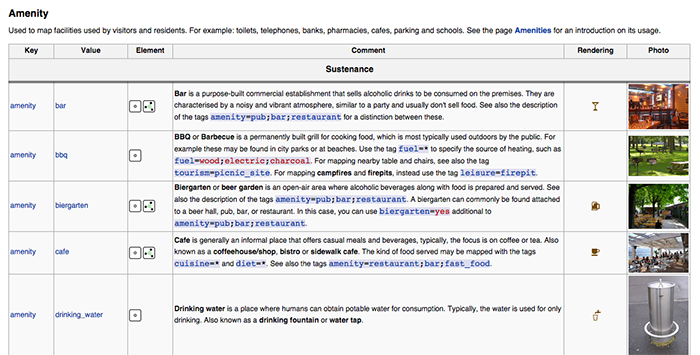
\includegraphics{figure/osm_mapfeatures.png}

\end{frame}

\begin{frame}{\href{https://wiki.openstreetmap.org/wiki/Tags}{Openstreetmap
Tags}}

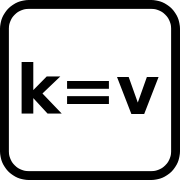
\includegraphics{figure/osm_tag.png}

\end{frame}

\begin{frame}{Objekttypen in OSM}

\begin{itemize}
\item
  Es gibt prinipiell drei verschiedene Objekttypen:
\item
\end{itemize}

\end{frame}

\begin{frame}{Download von OpenStreetMap Daten}

\begin{itemize}
\item
  \url{https://mapzen.com/} - Ausschnitte von OpenStreetMap für einzelne
  Städte (\href{https://mapzen.com/data/metro-extracts/}{metro
  extracts})
\item
  Über Geofabrik lassen sich aktuelle Ausschnitte (auch Shapefiles)
  herunterladen (\url{http://download.geofabrik.de/})
\item
  Kartendaten (\href{http://www.openaprs.net/}{\textbf{openaprs}})
\end{itemize}

\end{frame}

\begin{frame}[fragile]{Bei großen Datenmengen}

\begin{itemize}
\item
  Hier geht es nur um das Herunterladen kleiner Ausschnitte.
\item
  Wenn größere Datenmengen benötigt werden, sollte man eine
  Datenbanklösung finden.
\item
  \href{http://www.postgresql.org/}{PostgreSQL} hat den Vorteil, dass es
  Open-Source ist.
\item
  \href{http://www.postgresql.org/download/windows/}{Download PostreSQL}
\item
  \href{https://datashenanigan.wordpress.com/2015/05/18/getting-started-with-postgresql-in-r/}{Hier}
  ist eine Einführung in PostgreSQL zu finden
\item
  Sehr empfehlenswert: Arbeiten mit pgAdmin III
\item
  Beispiel: um Verknüpfung zu einer Datenbank herzustellen - Doppelklick
  auf den Server in pgAdmin III
\end{itemize}

\begin{block}{PostGIS für PostgreSQL}

\begin{itemize}
\tightlist
\item
  \href{http://postgis.net/install/}{\textbf{Installieren}} der PostGIS
  Erweiterung:
\end{itemize}

\begin{verbatim}
CREATE EXTENSION postgis;
\end{verbatim}

\end{block}

\end{frame}

\begin{frame}[fragile]{Programm zum Import der OSM Daten in PostgreSQL-
osm2pgsql}

\begin{itemize}
\tightlist
\item
  Läuft unter Linux deutlich besser
\item
  so könnte bspw. ein Import in PostgreSQL aussehen:
\end{itemize}

\begin{verbatim}
osm2pgsql -c -d osmBerlin --slim -C  -k  berlin-latest.osm.pbf
\end{verbatim}

\end{frame}

\begin{frame}{Nutze bspw. \href{http://www.qgis.org/de/site/}{QGIS} um
Shapefiles zu extrahieren}

\begin{itemize}
\tightlist
\item
  \href{http://www.qgistutorials.com/de/docs/downloading_osm_data.html}{Plugin
  OpenLayers}
\end{itemize}

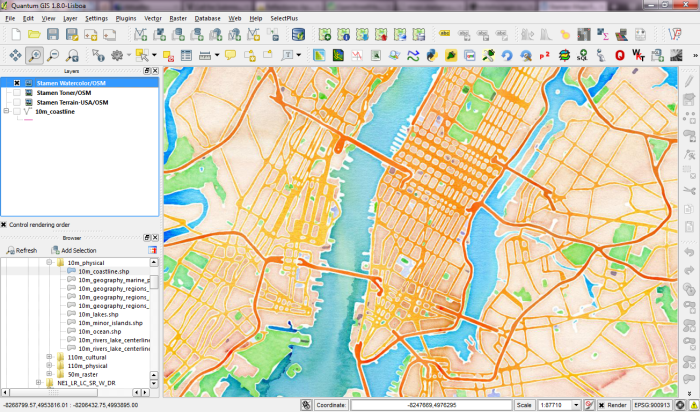
\includegraphics{figure/stamen_watercolor1.png}

\end{frame}

\begin{frame}{Links}

\begin{itemize}
\item
  \href{http://wiki.openstreetmap.org/wiki/Downloading_data}{\textbf{Wiki
  zum Downlaod}} von Openstreetmap Daten
\item
  \href{http://blog.openstreetmap.de/}{\textbf{Openstreetmap Blog}}
\item
  Liste möglicher Datenquellen für räumliche Analysen
  (\href{http://wiki.openstreetmap.org/wiki/Potential_Datasources}{weltweit}
  und in
  \href{http://wiki.openstreetmap.org/wiki/DE:Potential_Datasources}{\textbf{Deutschland}}
  )
\item
  \href{http://wiki.openstreetmap.org/wiki/SALB}{\textbf{SALB}} -
  Administrative Grenzen
\end{itemize}

\url{http://wiki.openstreetmap.org/wiki/SALB}

\end{frame}

\begin{frame}{Inhalt dieses Abschnitts}

\begin{itemize}
\tightlist
\item
  Das Konzept der Geokoordinaten erklären
\item
  Möglichkeiten vorstellen, die Geokodierung mit R durchzuführen
\end{itemize}

\end{frame}

\begin{frame}{Geokodierung}

\begin{block}{\href{https://github.com/adam-p/markdown-here/wiki/Markdown-Cheatsheet\#blockquotes}{Wikipedia
- Geocoding}}

\begin{quote}
Geocoding (\ldots{}) uses a description of a location, most typically a
postal address or place name, to find geographic coordinates from
spatial reference data \ldots{}
\end{quote}

\end{block}

\end{frame}

\begin{frame}[fragile]{Geokodierung mit dem Paket \texttt{ggmap}}

\begin{itemize}
\tightlist
\item
  Einer der ersten Ansätze Geokodierung mit R durchzuführen
\item
  Wenn Geokodierung mit R durchgeführt wird dieses Paket wohl am
  häufigsten verwendet.
\item
  Das führt auch dazu, dass im Internet zahlreiche Anwendungsbeispiele
  zu finden sind.
\end{itemize}

\begin{Shaded}
\begin{Highlighting}[]
\KeywordTok{library}\NormalTok{(ggmap)}
\KeywordTok{geocode}\NormalTok{(}\StringTok{"Heidelberg"}\NormalTok{)}
\end{Highlighting}
\end{Shaded}

\begin{verbatim}
Information from URL : http://maps.googleapis.com/maps/api/geocode/json?address=Heidelberg&sensor=false
       lon      lat
1 8.672434 49.39875
\end{verbatim}

\end{frame}

\begin{frame}{Latitude und Longitude}

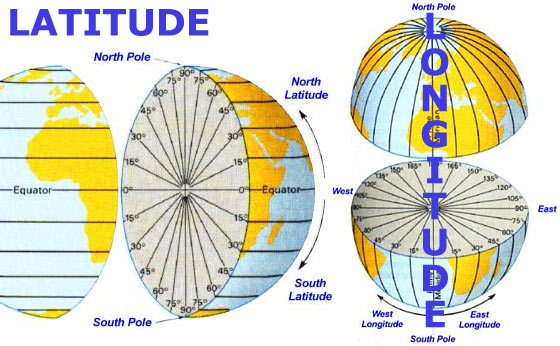
\includegraphics{figure/definition-of-latitude-longitude.jpg}

\href{http://modernsurvivalblog.com/survival-skills/basic-map-reading-latitude-longitude/}{http://modernsurvivalblog.com}

\end{frame}

\begin{frame}[fragile]{Die Distanz zwischen zwei Punkten}

\begin{Shaded}
\begin{Highlighting}[]
\KeywordTok{mapdist}\NormalTok{(}\StringTok{"Q1, 4 Mannheim"}\NormalTok{,}\StringTok{"B2, 1 Mannheim"}\NormalTok{)}
\end{Highlighting}
\end{Shaded}

\begin{Shaded}
\begin{Highlighting}[]
\KeywordTok{mapdist}\NormalTok{(}\StringTok{"Q1, 4 Mannheim"}\NormalTok{,}\StringTok{"B2, 1 Mannheim"}\NormalTok{,}\DataTypeTok{mode=}\StringTok{"walking"}\NormalTok{)}
\end{Highlighting}
\end{Shaded}

\begin{block}{Eine andere Distanz bekommen}

\begin{Shaded}
\begin{Highlighting}[]
\KeywordTok{mapdist}\NormalTok{(}\StringTok{"Q1, 4 Mannheim"}\NormalTok{,}\StringTok{"B2, 1 Mannheim"}\NormalTok{,}\DataTypeTok{mode=}\StringTok{"bicycling"}\NormalTok{)}
\end{Highlighting}
\end{Shaded}

\end{block}

\end{frame}

\begin{frame}[fragile]{Geokodierung mit dem Paket \texttt{tmaptools}}

\begin{itemize}
\tightlist
\item
  Beim Paket \texttt{tmaptools} wird die Nominatim API zur Geokodierung
  verwendet.
\item
  Diese Funktion hat den Vorteil, dass eine Projektion ausgewählt werden
  kann, in der die Geokodierungen zurück gegeben werden.
\end{itemize}

\begin{Shaded}
\begin{Highlighting}[]
\KeywordTok{library}\NormalTok{(}\StringTok{"tmaptools"}\NormalTok{)}
\end{Highlighting}
\end{Shaded}

\end{frame}

\begin{frame}[fragile]{Koordinaten verschiedener Orte in Deutschland}

\begin{Shaded}
\begin{Highlighting}[]
\NormalTok{cities <-}\StringTok{ }\KeywordTok{c}\NormalTok{(}\StringTok{"Hamburg"}\NormalTok{,}\StringTok{"Koeln"}\NormalTok{,}\StringTok{"Dresden"}\NormalTok{,}\StringTok{"Muenchen"}\NormalTok{)}

\NormalTok{lat <-}\StringTok{ }\KeywordTok{vector}\NormalTok{()}
\NormalTok{lon <-}\StringTok{ }\KeywordTok{vector}\NormalTok{()}
\ControlFlowTok{for}\NormalTok{ (i }\ControlFlowTok{in} \DecValTok{1}\OperatorTok{:}\KeywordTok{length}\NormalTok{(cities))\{}
\NormalTok{  gc <-}\StringTok{ }\KeywordTok{geocode_OSM}\NormalTok{(cities[i])}
\NormalTok{  lat[i] <-}\StringTok{ }\NormalTok{gc}\OperatorTok{$}\NormalTok{coords[}\DecValTok{1}\NormalTok{]}
\NormalTok{  lon[i] <-}\StringTok{ }\NormalTok{gc}\OperatorTok{$}\NormalTok{coords[}\DecValTok{2}\NormalTok{]}
\NormalTok{\}}
\end{Highlighting}
\end{Shaded}

\end{frame}

\begin{frame}[fragile]{Welche Koordinaten hat der Norden}

\begin{Shaded}
\begin{Highlighting}[]
\NormalTok{Dat <-}\StringTok{ }\KeywordTok{data.frame}\NormalTok{(cities,lon,lat)}
\KeywordTok{kable}\NormalTok{(Dat)}
\end{Highlighting}
\end{Shaded}

\begin{longtable}[]{@{}lrr@{}}
\toprule
cities & lon & lat\tabularnewline
\midrule
\endhead
Hamburg & 53.55034 & 10.000654\tabularnewline
Koeln & 50.93836 & 6.959974\tabularnewline
Dresden & 51.04933 & 13.738144\tabularnewline
Muenchen & 48.13711 & 11.575382\tabularnewline
\bottomrule
\end{longtable}

\end{frame}

\begin{frame}{Geokodierung - verschiedene Punkte von Interesse}

\end{frame}

\begin{frame}[fragile]{Punkte in der Karte}

\begin{Shaded}
\begin{Highlighting}[]
\NormalTok{MA_map <-}\StringTok{ }\KeywordTok{qmap}\NormalTok{(}\StringTok{"Mannheim"}\NormalTok{)}
\end{Highlighting}
\end{Shaded}

\begin{Shaded}
\begin{Highlighting}[]
\NormalTok{MA_map }\OperatorTok{+}
\KeywordTok{geom_point}\NormalTok{(}\KeywordTok{aes}\NormalTok{(}\DataTypeTok{x =}\NormalTok{ x, }\DataTypeTok{y =}\NormalTok{ y),}
\DataTypeTok{data =}\NormalTok{ ListPOI)}
\end{Highlighting}
\end{Shaded}

\end{frame}

\begin{frame}[fragile]{Punkte in der Karte}

\begin{Shaded}
\begin{Highlighting}[]
\NormalTok{MA_map }\OperatorTok{+}
\KeywordTok{geom_point}\NormalTok{(}\KeywordTok{aes}\NormalTok{(}\DataTypeTok{x =}\NormalTok{ x, }\DataTypeTok{y =}\NormalTok{ y),}\DataTypeTok{col=}\StringTok{"red"}\NormalTok{,}
\DataTypeTok{data =}\NormalTok{ ListPOI)}
\end{Highlighting}
\end{Shaded}

\end{frame}

\begin{frame}[fragile]{Reverse Geokodierung}

\begin{quote}
Reverse geocoding is the process of back (reverse) coding of a point
location (latitude, longitude) to a readable address or place name. This
permits the identification of nearby street addresses, places, and/or
areal subdivisions such as neighbourhoods, county, state, or country.
\end{quote}

Quelle:
\href{https://en.wikipedia.org/wiki/Reverse_geocoding}{Wikipedia}

\begin{Shaded}
\begin{Highlighting}[]
\KeywordTok{revgeocode}\NormalTok{(}\KeywordTok{c}\NormalTok{(}\DecValTok{48}\NormalTok{,}\DecValTok{8}\NormalTok{))}
\end{Highlighting}
\end{Shaded}

\end{frame}

\begin{frame}[fragile]{Daten einlesen}

\begin{itemize}
\tightlist
\item
  Hier wird ein Beispieldatensatz eingelesen, den ich über räumliche
  Stichproben und reverse geocoding erzeugt habe.
\end{itemize}

\begin{Shaded}
\begin{Highlighting}[]
\KeywordTok{load}\NormalTok{(}\StringTok{"../data/addr_list_t_68239.RData"}\NormalTok{)}
\KeywordTok{head}\NormalTok{(addr_list_t)}
\end{Highlighting}
\end{Shaded}

\begin{verbatim}
## [1] "Lilienstraße 32A, 68535 Edingen-Neckarhausen, Germany"
## [2] "Waldspitze 6, 68239 Mannheim, Germany"                
## [3] "Holzweg 51, 68239 Mannheim, Germany"                  
## [4] "Kloppenheimer Str. 247, 68239 Mannheim, Germany"      
## [5] "Mallaustraße 121, 68219 Mannheim, Germany"            
## [6] "Holzweg 33A, 68239 Mannheim, Germany"
\end{verbatim}

\end{frame}

\begin{frame}[fragile]{Die erste Adressen geokodieren}

\begin{Shaded}
\begin{Highlighting}[]
\KeywordTok{geocode_OSM}\NormalTok{(addr_list_t[}\DecValTok{1}\NormalTok{])}
\end{Highlighting}
\end{Shaded}

\begin{verbatim}
## $query
## [1] "Lilienstraße 32A, 68535 Edingen-Neckarhausen, Germany"
## 
## $coords
##         x         y 
##  8.584601 49.445360 
## 
## $bbox
##         min       max
## x  8.584494  8.584708
## y 49.445276 49.445443
\end{verbatim}

\end{frame}

\begin{frame}[fragile]{Alle Adressen geokodieren}

\begin{Shaded}
\begin{Highlighting}[]
\NormalTok{gc_list <-}\StringTok{ }\KeywordTok{list}\NormalTok{()}

\ControlFlowTok{for}\NormalTok{ (i }\ControlFlowTok{in} \DecValTok{1}\OperatorTok{:}\KeywordTok{length}\NormalTok{(addr_list_t))\{}
\NormalTok{  gc_list[[i]] <-}\StringTok{ }\KeywordTok{geocode_OSM}\NormalTok{(addr_list_t[i])}
\NormalTok{\}}
\end{Highlighting}
\end{Shaded}

\end{frame}

\begin{frame}[fragile]{Geokodierung mit dem R-Paket \texttt{opencage}}

\begin{itemize}
\tightlist
\item
  Um dieses Paket zu nutzen muss man sich vorher bei der API
  registrieren
\end{itemize}

\begin{Shaded}
\begin{Highlighting}[]
\KeywordTok{library}\NormalTok{(opencage)}
\end{Highlighting}
\end{Shaded}

\begin{Shaded}
\begin{Highlighting}[]
\NormalTok{gc_info<-}\KeywordTok{opencage_forward}\NormalTok{(}\DataTypeTok{placename =} 
                              \StringTok{"Amsterdam, Van Woustraat"}\NormalTok{)}
\end{Highlighting}
\end{Shaded}

\begin{itemize}
\tightlist
\item
  Hinweise, wie das Paket genutzt erden kann sind im
  \href{https://ropensci.org/tutorials/opencage_tutorial/}{\textbf{opencage
  Tutorial}} zu finden.
\end{itemize}

\end{frame}

\begin{frame}[fragile]{Das Paket
\href{https://github.com/ropensci/geonames}{\texttt{geonames}}}

\begin{Shaded}
\begin{Highlighting}[]
\KeywordTok{install.packages}\NormalTok{(}\StringTok{"geonames"}\NormalTok{)}
\end{Highlighting}
\end{Shaded}

\begin{itemize}
\tightlist
\item
  Ein Account ist notwendig um die meisten Funktionen des Paketes
  \texttt{geonames}zu nutzen.
\end{itemize}

\begin{Shaded}
\begin{Highlighting}[]
\KeywordTok{library}\NormalTok{(geonames)}
\end{Highlighting}
\end{Shaded}

\begin{Shaded}
\begin{Highlighting}[]
\KeywordTok{options}\NormalTok{(}\DataTypeTok{geonamesUsername=}\StringTok{"myusername"}\NormalTok{)}
\end{Highlighting}
\end{Shaded}

\begin{Shaded}
\begin{Highlighting}[]
\NormalTok{MAwiki<-}\KeywordTok{GNfindNearbyWikipedia}\NormalTok{(}\DataTypeTok{postalcode=}\DecValTok{68239}\NormalTok{,}\DataTypeTok{country=}\StringTok{"DE"}\NormalTok{,}
                              \DataTypeTok{radius=}\DecValTok{10}\NormalTok{)}
\end{Highlighting}
\end{Shaded}

\end{frame}

\begin{frame}[fragile]{Wikipediaeinträge in der Nähe}

\begin{longtable}[]{@{}lllllllllllll@{}}
\toprule
elevation & feature & lng & distance & countryCode & rank & lang & title
& lat & wikipediaUrl & summary & thumbnailImg & geoNameId\tabularnewline
\midrule
\endhead
102 & city & 8.46711 & 0.1738 & DE & 98 & en & Quadratestadt & 49.48848
& en.wikipedia.org/wiki/Quadratestadt & NA & NA & NA\tabularnewline
103 & landmark & 8.46212 & 0.1986 & NA & 90 & en & Reiss Engelhorn
Museum & 49.48888 & en.wikipedia.org/wiki/Reiss\_Engelhorn\_Museum & The
Reiss Engelhorn Museum, or (rem for short), is a museum in Mannheim,
Germany. They have an exhibition area of , and house around 1.2 million
objects. They are one of the largest publicly-owned museums in southern
Germany (\ldots{}) &
\url{http://www.geonames.org/img/wikipedia/29000/thumb-28652-100.jpg} &
NA\tabularnewline
103 & landmark & 8.4616 & 0.2423 & DE & 13 & en & Klapsmühl' am Rathaus
& 49.4891 &
en.wikipedia.org/wiki/Klapsm\%C3\%BChl\%E2\%80\%99\_am\_Rathaus &
Klapsmühl' am Rathaus is a theatre in Baden-Württemberg, Germany. & NA &
NA\tabularnewline
104 & landmark & 8.46294 & 0.3178 & DE & 84 & en & GESIS -- Leibniz
Institute for the Social Sciences & 49.485686 &
en.wikipedia.org/wiki/GESIS\_\%E2\%80\%93\_Leibniz\_Institute\_for\_the\_Social\_Sciences
& The GESIS -- Leibniz-Institute for the Social Sciences headquartered
in Mannheim with locations in Cologne and Berlin is the largest German
infrastructure institute for the Social Sciences. With basic
research-based services and consulting covering all levels of the
scientific process GESIS supports (\ldots{}) & NA & NA\tabularnewline
102 & city & 8.4691 & 0.3258 & DE & 100 & en & Mannheim & 49.489 &
en.wikipedia.org/wiki/Mannheim & Mannheim (listen, Palatine German:
Monnem or Mannem) is a city in the southwestern part of Germany, the
third-largest in the German state of Baden-Württemberg after Stuttgart
and Karlsruhe. Mannheim is among the twenty largest cities in Germany,
with a 2012 population of approximately 295,000 (\ldots{}) & NA &
2873891\tabularnewline
\bottomrule
\end{longtable}

\begin{itemize}
\item
  \href{http://www.geonames.org/login}{Login für Geonames}
\item
  \href{http://www.geonames.org/enablefreewebservice}{Link um mit den
  Geodaten zu arbeiten}
\item
  \href{http://www.geonames.org/export/ws-overview.html}{Informationen
  über den Download}
\end{itemize}

\begin{Shaded}
\begin{Highlighting}[]
\KeywordTok{library}\NormalTok{(osmdata)}
\NormalTok{bbox <-}\StringTok{ }\KeywordTok{getbb}\NormalTok{(}\StringTok{"Mannheim"}\NormalTok{)}
\end{Highlighting}
\end{Shaded}

\begin{Shaded}
\begin{Highlighting}[]
\NormalTok{erg <-}\StringTok{ }\NormalTok{geonames}\OperatorTok{::}\KeywordTok{GNcities}\NormalTok{(}\FloatTok{49.649591}\NormalTok{,}\FloatTok{8.627236}\NormalTok{,}
                          \FloatTok{49.329591}\NormalTok{,}\FloatTok{8.307236}\NormalTok{)}
\end{Highlighting}
\end{Shaded}

\end{frame}

\begin{frame}[fragile]{Das Paket \texttt{googleway}}

\begin{quote}
Accesses Google Maps APIs to Retrieve Data and Plot Maps
\end{quote}

\begin{Shaded}
\begin{Highlighting}[]
\KeywordTok{library}\NormalTok{(googleway)}
\end{Highlighting}
\end{Shaded}

\begin{itemize}
\tightlist
\item
  Ein API Schlüssel ist notwendig um die meisten Funktionen des Paketes
  zu nutzen.
\end{itemize}

\end{frame}

\begin{frame}[fragile]{Das Paket \texttt{bbox}}

\begin{itemize}
\item
  Das Paket \texttt{bbox} ist auf github zu finden.
\item
  Beispieldatensatz laden:
\end{itemize}

\begin{Shaded}
\begin{Highlighting}[]
\KeywordTok{load}\NormalTok{(}\StringTok{"../data/ddat.RData"}\NormalTok{)}
\end{Highlighting}
\end{Shaded}

\begin{itemize}
\tightlist
\item
  Rahmen für das räumliche Objekt bestimmen:
\end{itemize}

\begin{Shaded}
\begin{Highlighting}[]
\KeywordTok{library}\NormalTok{(bbox)}
\KeywordTok{b_box}\NormalTok{(ddat)}
\end{Highlighting}
\end{Shaded}

\begin{verbatim}
## [1]  5.866286 47.273602 15.048632 55.058262
\end{verbatim}

\begin{Shaded}
\begin{Highlighting}[]
\KeywordTok{citation}\NormalTok{(}\StringTok{"bbox"}\NormalTok{)}
\end{Highlighting}
\end{Shaded}

\end{frame}

\begin{frame}[fragile]{Links}

\begin{itemize}
\item
  Überblick von Jesse Sadler zur
  \href{https://www.jessesadler.com/post/geocoding-with-r/}{\textbf{Geokodierung
  mit R}}
\item
  Ein Schummelzettel für
  \href{https://www.nceas.ucsb.edu/~frazier/RSpatialGuides/ggmap/ggmapCheatsheet.pdf}{\textbf{\texttt{ggmap}}}
\item
  Die Vignette zum Paket \texttt{tmap} -
  \href{https://cran.r-project.org/web/packages/tmap/vignettes/tmap-getstarted.html}{\textbf{tmap:
  get started}}
\item
  \href{https://www.latlong.net/place/hamburg-germany-8766.html}{\textbf{latlong.net}}
  - eine Homepage um Koordinaaten zu bestimmen.
\end{itemize}

\end{frame}

\begin{frame}{\href{http://www.openstreetmap.org/export}{OSM Ausschnitte
herunterladen}}

\textless{}www.openstreetmap.org/export\textgreater{}

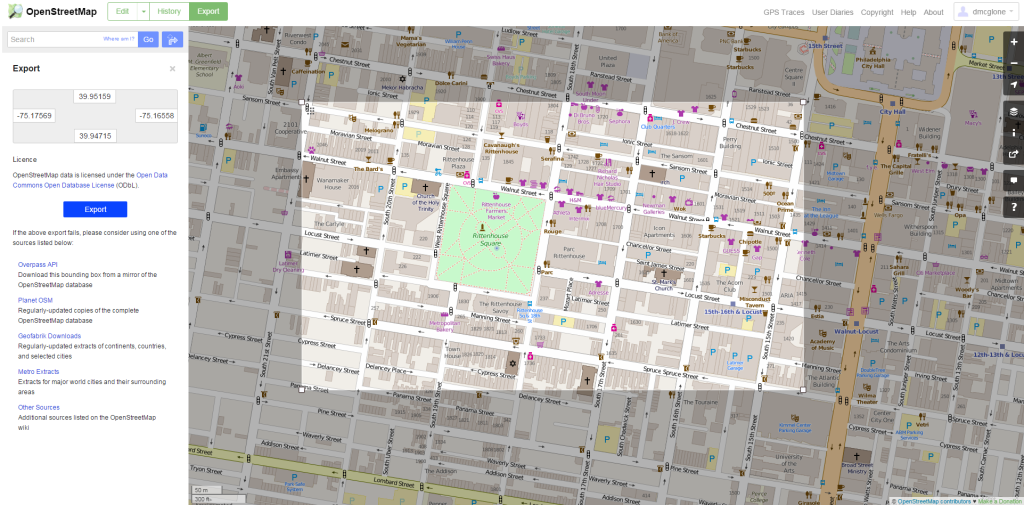
\includegraphics{figure/openstreetmap_export-1024x505.png}

\end{frame}

\begin{frame}[fragile]{Das R-Paket \texttt{XML} - Gaston Sanchez}

\begin{Shaded}
\begin{Highlighting}[]
\KeywordTok{library}\NormalTok{(}\StringTok{"XML"}\NormalTok{)}
\end{Highlighting}
\end{Shaded}

\begin{block}{Gaston Sanchez - Dataflow}

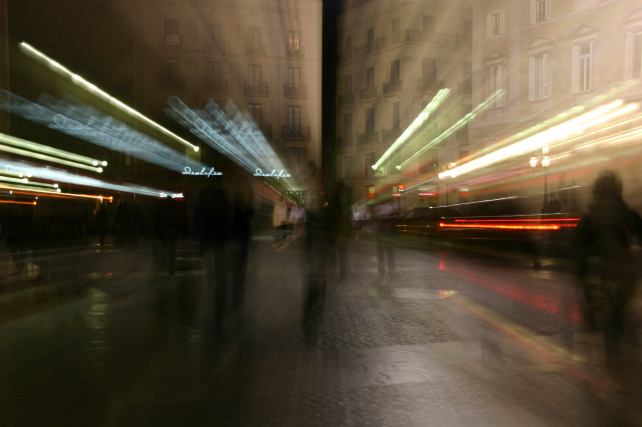
\includegraphics{figure/GastonSanchez2.png}

Seine Arbeit sieht man \href{http://gastonsanchez.com/}{\textbf{hier}}.

\end{block}

\end{frame}

\begin{frame}{\href{https://github.com/gastonstat/tutorial-R-web-data/blob/master/04-parsing-xml/04-parsing-xml.pdf}{Das
Arbeiten mit XML Daten}}

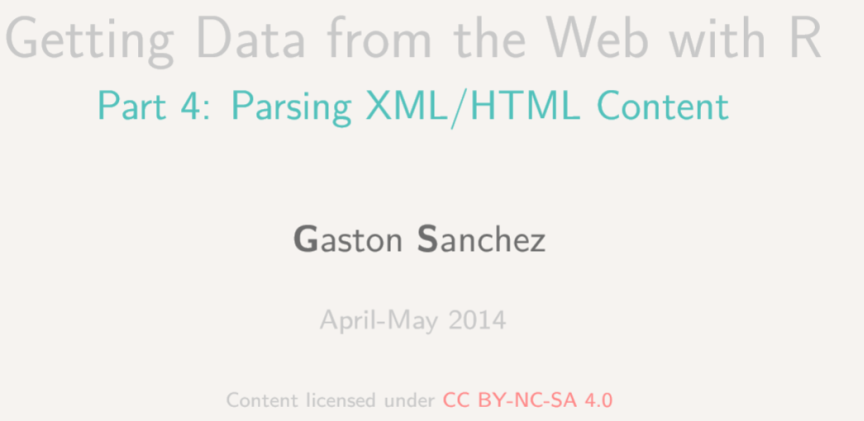
\includegraphics{figure/GastonSanchez3.PNG}

\end{frame}

\begin{frame}{Funktionen im XML Paket}

\begin{longtable}[]{@{}ll@{}}
\toprule
Function & Description\tabularnewline
\midrule
\endhead
xmlName() & name of the node\tabularnewline
xmlSize() & number of subnodes\tabularnewline
xmlAttrs() & named character vector of all attributes\tabularnewline
xmlGetAttr() & value of a single attribute\tabularnewline
xmlValue() & contents of a leaf node\tabularnewline
xmlParent() & name of parent node\tabularnewline
xmlAncestors() & name of ancestor nodes\tabularnewline
getSibling() & siblings to the right or to the left\tabularnewline
xmlNamespace() & the namespace (if there's one)\tabularnewline
\bottomrule
\end{longtable}

\end{frame}

\begin{frame}{\href{http://www.openstreetmap.org/export}{Einzelne
Objekte finden}}

\textless{}www.openstreetmap.org/export\textgreater{}

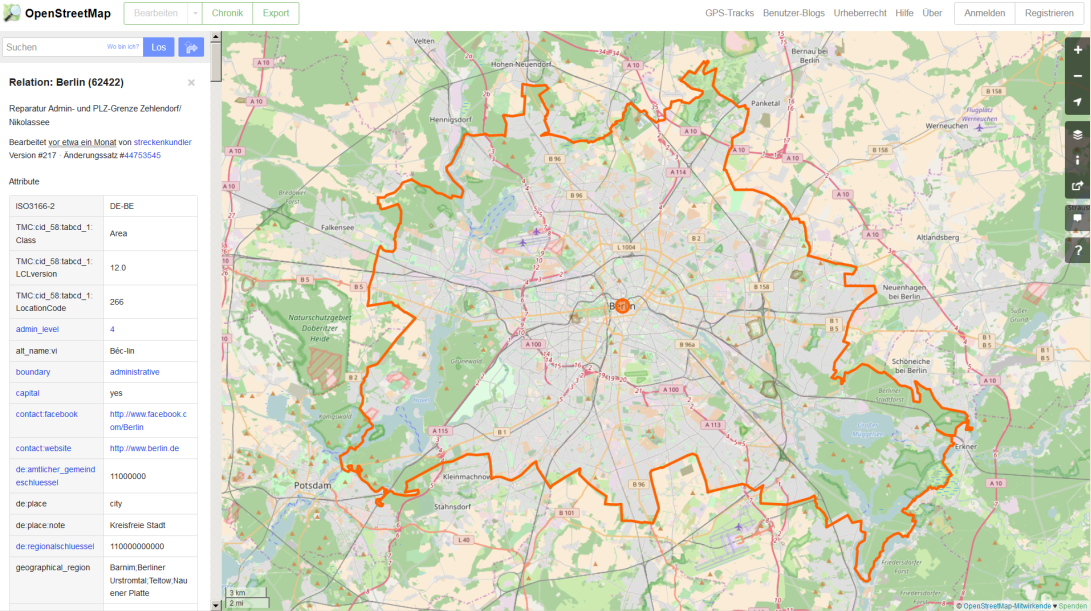
\includegraphics{figure/admgrBer.PNG}

\end{frame}

\begin{frame}[fragile]{Beispiel: administrative Grenzen Berlin}

\href{http://wiki.openstreetmap.org/wiki/DE:Grenze\#Bundesl.C3.A4ndergrenze_-_admin_level.3D4}{Administrative
Grenzen für Deutschland}

\begin{Shaded}
\begin{Highlighting}[]
\NormalTok{url <-}\StringTok{ "https://api.openstreetmap.org/api/0.6/relation/62422"}
\end{Highlighting}
\end{Shaded}

\begin{Shaded}
\begin{Highlighting}[]
\NormalTok{BE <-}\StringTok{ }\KeywordTok{xmlParse}\NormalTok{(url)}
\end{Highlighting}
\end{Shaded}

\begin{Shaded}
\begin{Highlighting}[]
\NormalTok{BE <-}\StringTok{ }\KeywordTok{xmlParse}\NormalTok{(}\StringTok{"../data/62422.xml"}\NormalTok{)}
\end{Highlighting}
\end{Shaded}

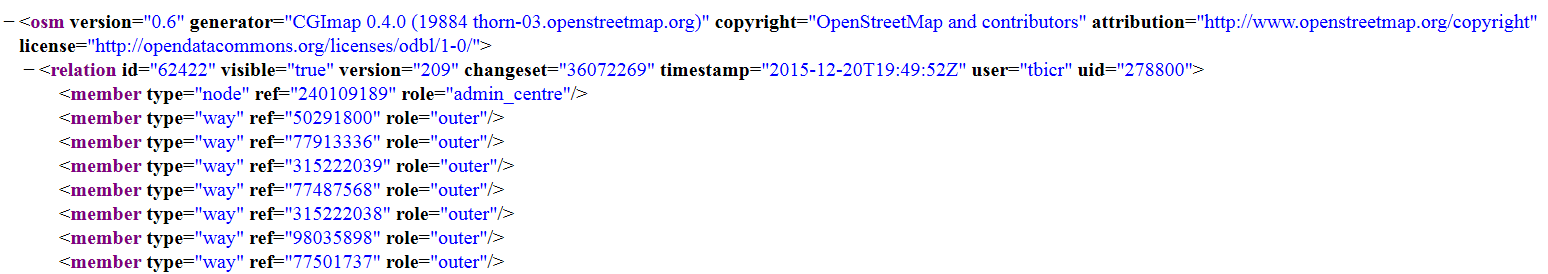
\includegraphics{figure/ExampleAdmBE.PNG}

\end{frame}

\begin{frame}[fragile]{Das XML analysieren}

\begin{itemize}
\tightlist
\item
  \href{http://www.informit.com/articles/article.aspx?p=2215520}{Tobi
  Bosede - Working with XML Data in R}
\end{itemize}

\begin{Shaded}
\begin{Highlighting}[]
\NormalTok{xmltop =}\StringTok{ }\KeywordTok{xmlRoot}\NormalTok{(BE)}
\KeywordTok{class}\NormalTok{(xmltop)}
\end{Highlighting}
\end{Shaded}

\begin{verbatim}
## [1] "XMLInternalElementNode" "XMLInternalNode"       
## [3] "XMLAbstractNode"
\end{verbatim}

\begin{Shaded}
\begin{Highlighting}[]
\KeywordTok{xmlSize}\NormalTok{(xmltop)}
\end{Highlighting}
\end{Shaded}

\begin{verbatim}
## [1] 1
\end{verbatim}

\begin{Shaded}
\begin{Highlighting}[]
\KeywordTok{xmlSize}\NormalTok{(xmltop[[}\DecValTok{1}\NormalTok{]])}
\end{Highlighting}
\end{Shaded}

\begin{verbatim}
## [1] 337
\end{verbatim}

\end{frame}

\begin{frame}[fragile]{Nutzung von Xpath}

\begin{quote}
\href{https://de.wikipedia.org/wiki/XPath}{Xpath}, the XML Path
Language, is a query language for selecting nodes from an XML document.
\end{quote}

\begin{Shaded}
\begin{Highlighting}[]
\KeywordTok{xpathApply}\NormalTok{(BE,}\StringTok{"//tag[@k = 'population']"}\NormalTok{)}
\end{Highlighting}
\end{Shaded}

\begin{verbatim}
## [[1]]
## <tag k="population" v="3440441"/> 
## 
## attr(,"class")
## [1] "XMLNodeSet"
\end{verbatim}

\end{frame}

\begin{frame}[fragile]{Quelle für die Bevölkerungsgröße}

\begin{Shaded}
\begin{Highlighting}[]
\KeywordTok{xpathApply}\NormalTok{(BE,}\StringTok{"//tag[@k = 'source:population']"}\NormalTok{)}
\end{Highlighting}
\end{Shaded}

\begin{verbatim}
## [[1]]
## <tag k="source:population" v="http://www.statistik-berlin-brandenburg.de/Publikationen/Stat_Berichte/2010/SB_A1-1_A2-4_q01-10_BE.pdf 2010-10-01"/> 
## 
## attr(,"class")
## [1] "XMLNodeSet"
\end{verbatim}

-\href{https://www.statistik-berlin-brandenburg.de/datenbank/inhalt-datenbank.asp}{\textbf{Statistik
Berlin Brandenburg}}

\end{frame}

\begin{frame}[fragile]{Etwas überraschend:}

\begin{Shaded}
\begin{Highlighting}[]
\KeywordTok{xpathApply}\NormalTok{(BE,}\StringTok{"//tag[@k = 'name:ta']"}\NormalTok{)}
\end{Highlighting}
\end{Shaded}

\begin{verbatim}
## [[1]]
## <tag k="name:ta" v="<U+0BAA><U+0BC6><U+0BB0><U+0BCD><U+0BB2><U+0BBF><U+0BA9><U+0BCD>"/> 
## 
## attr(,"class")
## [1] "XMLNodeSet"
\end{verbatim}

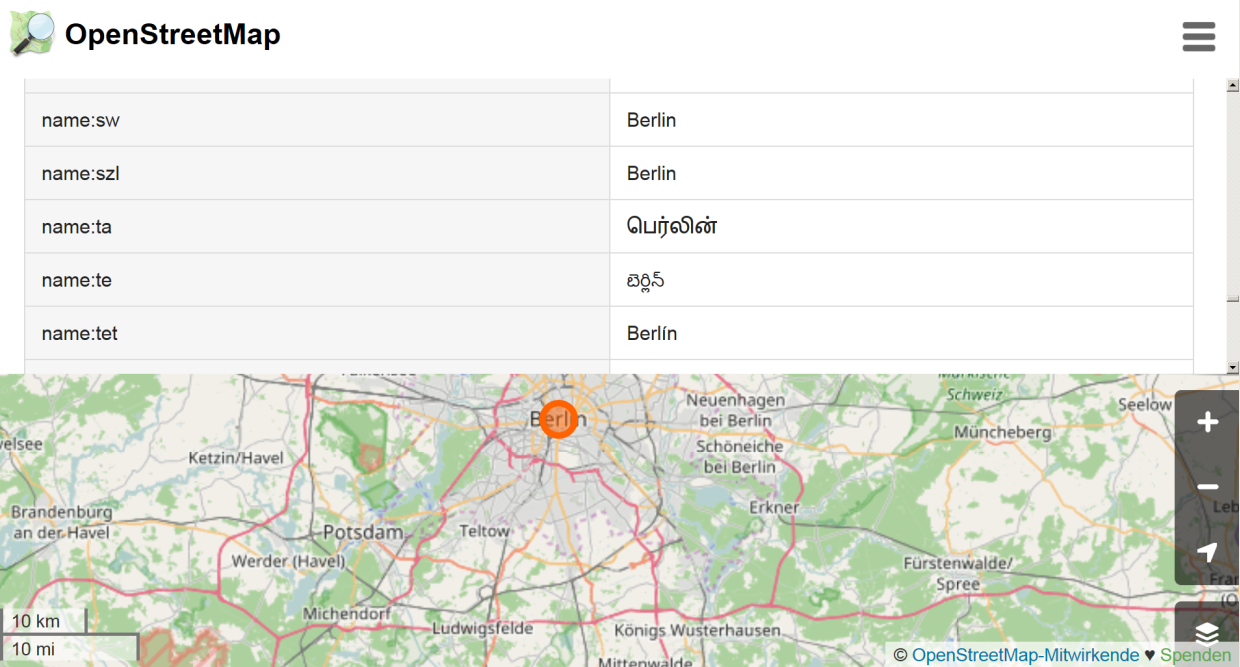
\includegraphics{figure/OSMBerta.png}

\end{frame}

\begin{frame}[fragile]{Geographische Region}

\begin{Shaded}
\begin{Highlighting}[]
\NormalTok{region <-}\StringTok{ }\KeywordTok{xpathApply}\NormalTok{(BE,}
  \StringTok{"//tag[@k = 'geographical_region']"}\NormalTok{)}
\CommentTok{# regular expressions}
\NormalTok{region[[}\DecValTok{1}\NormalTok{]]}
\end{Highlighting}
\end{Shaded}

\begin{verbatim}
## <tag k="geographical_region" v="Barnim;Berliner Urstromtal;Teltow;Nauener Platte"/>
\end{verbatim}

\begin{verbatim}
<tag k="geographical_region" 
  v="Barnim;Berliner Urstromtal;
  Teltow;Nauener Platte"/>
\end{verbatim}

\end{frame}

\begin{frame}{Landkreis}

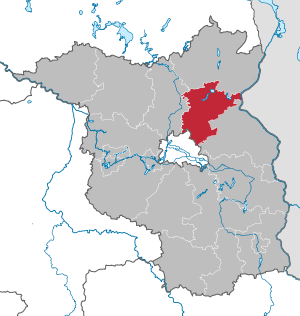
\includegraphics{figure/Barnim.png}

\end{frame}

\begin{frame}[fragile]{Weiteres Beispiel}

\begin{Shaded}
\begin{Highlighting}[]
\NormalTok{url2<-}\StringTok{"http://api.openstreetmap.org/api/0.6/node/25113879"}
\NormalTok{obj2<-}\KeywordTok{xmlParse}\NormalTok{(url2)}
\NormalTok{obj_amenity<-}\KeywordTok{xpathApply}\NormalTok{(obj2,}\StringTok{"//tag[@k = 'amenity']"}\NormalTok{)[[}\DecValTok{1}\NormalTok{]]}
\NormalTok{obj_amenity}
\end{Highlighting}
\end{Shaded}

\begin{verbatim}
## <tag k="amenity" v="university"/>
\end{verbatim}

\end{frame}

\begin{frame}[fragile]{Wikipedia Artikel}

\begin{Shaded}
\begin{Highlighting}[]
\KeywordTok{xpathApply}\NormalTok{(obj2,}\StringTok{"//tag[@k = 'wikipedia']"}\NormalTok{)[[}\DecValTok{1}\NormalTok{]]}
\end{Highlighting}
\end{Shaded}

\begin{verbatim}
## <tag k="wikipedia" v="de:Universität Mannheim"/>
\end{verbatim}

\begin{Shaded}
\begin{Highlighting}[]
\KeywordTok{xpathApply}\NormalTok{(obj2,}\StringTok{"//tag[@k = 'wheelchair']"}\NormalTok{)[[}\DecValTok{1}\NormalTok{]]}
\end{Highlighting}
\end{Shaded}

\begin{Shaded}
\begin{Highlighting}[]
\KeywordTok{xpathApply}\NormalTok{(obj2,}\StringTok{"//tag[@k = 'name']"}\NormalTok{)[[}\DecValTok{1}\NormalTok{]]}
\end{Highlighting}
\end{Shaded}

\end{frame}

\begin{frame}[fragile]{Das C und das A}

\begin{Shaded}
\begin{Highlighting}[]
\NormalTok{url3<-}\StringTok{"http://api.openstreetmap.org/api/0.6/node/303550876"}
\NormalTok{obj3 <-}\StringTok{ }\KeywordTok{xmlParse}\NormalTok{(url3)}
\KeywordTok{xpathApply}\NormalTok{(obj3,}\StringTok{"//tag[@k = 'opening_hours']"}\NormalTok{)[[}\DecValTok{1}\NormalTok{]]}
\end{Highlighting}
\end{Shaded}

\begin{verbatim}
## <tag k="opening_hours" v="Mo-Sa 09:00-20:00; Su,PH off"/>
\end{verbatim}

\end{frame}

\begin{frame}[fragile]{Hin und weg}

\begin{Shaded}
\begin{Highlighting}[]
\NormalTok{url4<-}\StringTok{"http://api.openstreetmap.org/api/0.6/node/25439439"}
\NormalTok{obj4 <-}\StringTok{ }\KeywordTok{xmlParse}\NormalTok{(url4)}
\KeywordTok{xpathApply}\NormalTok{(obj4,}\StringTok{"//tag[@k = 'railway:station_category']"}\NormalTok{)[[}\DecValTok{1}\NormalTok{]]}
\end{Highlighting}
\end{Shaded}

\begin{verbatim}
## <tag k="railway:station_category" v="2"/>
\end{verbatim}

\begin{itemize}
\tightlist
\item
  \href{https://de.wikipedia.org/wiki/Bahnhofskategorie}{\textbf{Wikipedia
  Artikel Bahnhofskategorien}}
\end{itemize}

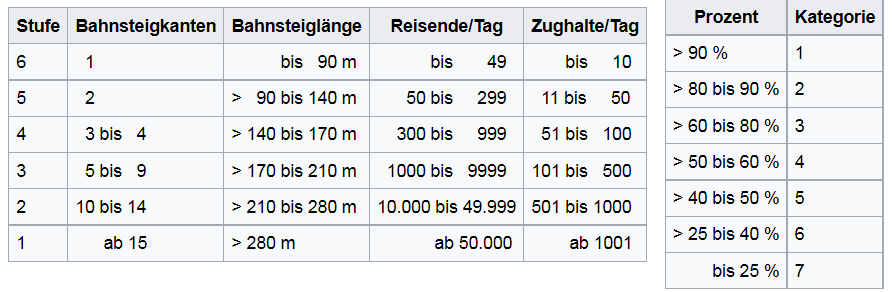
\includegraphics{figure/Bahnhofskategorien.PNG}

\end{frame}

\begin{frame}[fragile]{Exkurs: Bahnhofskategorien}

\begin{itemize}
\tightlist
\item
  \href{https://cran.r-project.org/web/packages/rvest/index.html}{\textbf{rvest:
  Easily Harvest (Scrape) Web Pages}}
\end{itemize}

\begin{Shaded}
\begin{Highlighting}[]
\KeywordTok{library}\NormalTok{(rvest)}
\NormalTok{bhfkat<-}\KeywordTok{read_html}\NormalTok{(}
  \StringTok{"https://de.wikipedia.org/wiki/Bahnhofskategorie"}\NormalTok{)}
\NormalTok{df_html_bhfkat<-}\KeywordTok{html_table}\NormalTok{(}
  \KeywordTok{html_nodes}\NormalTok{(bhfkat, }\StringTok{"table"}\NormalTok{)[[}\DecValTok{2}\NormalTok{]],}\DataTypeTok{fill =} \OtherTok{TRUE}\NormalTok{)}
\end{Highlighting}
\end{Shaded}

\end{frame}

\begin{frame}{Bahnhofskategorien Übersicht}

\begin{longtable}[]{@{}lllllll@{}}
\toprule
Stufe & Bahnsteigkanten & Bahnsteiglänge{[}Anm 1{]} & Reisende/Tag &
Zughalte/Tag & Service{[}Anm 2{]} & Stufenfreiheit{[}Anm
3{]}\tabularnewline
\midrule
\endhead
(0) & --- & --- & --- & --- & Nein & Nein\tabularnewline
1 & 01 & \textgreater{} 000 bis 090 m & 00.000 bis 00.049 & 000 bis 0010
& Ja & Ja\tabularnewline
2 & 02 & \textgreater{} 090 bis 140 m & 00.050 bis 00.299 & 011 bis 0050
& --- & ---\tabularnewline
3 & 03 bis 04 & \textgreater{} 140 bis 170 m & 00.300 bis 0.0999 & 051
bis 0100 & --- & ---\tabularnewline
4 & 05 bis 09 & \textgreater{} 170 bis 210 m & 01.000 bis 09.999 & 101
bis 0500 & --- & ---\tabularnewline
5 & 10 bis 14 & \textgreater{} 210 bis 280 m & 10.000 bis 49.999 & 501
bis 1000 & --- & ---\tabularnewline
6 & 00i ab 15 & \textgreater{} 280 m bis 000 & 000000 ab 50.000 & 000i
ab 1001 & --- & ---\tabularnewline
Gewichtung & 20~\% & 20~\% & 20~\% & 20~\% & 15~\% & 5~\%\tabularnewline
\bottomrule
\end{longtable}

\end{frame}

\begin{frame}[fragile]{Nur fliegen ist schöner}

\begin{Shaded}
\begin{Highlighting}[]
\NormalTok{url5<-}\StringTok{"http://api.openstreetmap.org/api/0.6/way/162149882"}
\NormalTok{obj5<-}\KeywordTok{xmlParse}\NormalTok{(url5)}
\KeywordTok{xpathApply}\NormalTok{(obj5,}\StringTok{"//tag[@k = 'name']"}\NormalTok{)[[}\DecValTok{1}\NormalTok{]]}
\end{Highlighting}
\end{Shaded}

\begin{verbatim}
## <tag k="name" v="City-Airport Mannheim"/>
\end{verbatim}

\begin{Shaded}
\begin{Highlighting}[]
\KeywordTok{xpathApply}\NormalTok{(obj5,}\StringTok{"//tag[@k = 'website']"}\NormalTok{)[[}\DecValTok{1}\NormalTok{]]}
\end{Highlighting}
\end{Shaded}

\begin{verbatim}
## <tag k="website" v="http://www.flugplatz-mannheim.de/"/>
\end{verbatim}

\begin{Shaded}
\begin{Highlighting}[]
\KeywordTok{xpathApply}\NormalTok{(obj5,}\StringTok{"//tag[@k = 'iata']"}\NormalTok{)[[}\DecValTok{1}\NormalTok{]]}
\end{Highlighting}
\end{Shaded}

\begin{verbatim}
## <tag k="iata" v="MHG"/>
\end{verbatim}

\end{frame}

\begin{frame}[fragile]{Das Paket \texttt{osmar} benutzen}

\begin{Shaded}
\begin{Highlighting}[]
\KeywordTok{library}\NormalTok{(}\StringTok{"osmar"}\NormalTok{)}
\NormalTok{node_ <-}\StringTok{ }\KeywordTok{xmlParse}\NormalTok{(}\StringTok{"../data/162149882.xml"}\NormalTok{)}
\NormalTok{node_osmar <-}\StringTok{ }\KeywordTok{as_osmar}\NormalTok{(node_)}
\NormalTok{node_osmar}
\end{Highlighting}
\end{Shaded}

\begin{verbatim}
## osmar object
## 0 nodes, 1 ways, 0 relations
\end{verbatim}

\end{frame}

\begin{frame}{\href{https://www.earthdatascience.org/courses/earth-analytics/spatial-data-r/intro-vector-data-r/}{Drei
Typen von Vektorobjekten}}

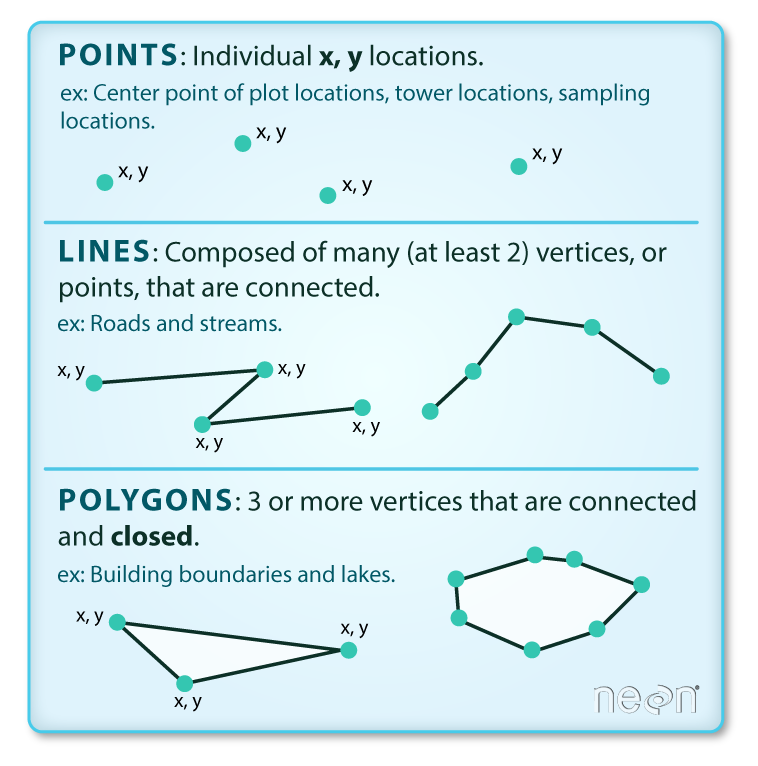
\includegraphics{figure/points-lines-polygons-vector-data-types.png}

\end{frame}

\begin{frame}{Die Ausdehnung}

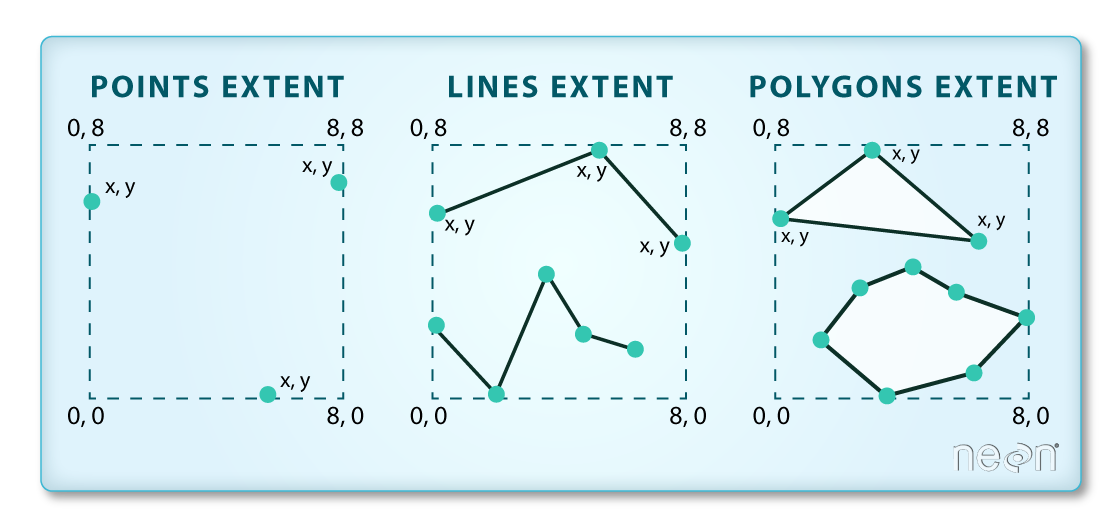
\includegraphics{figure/spatial-extent.png}

\end{frame}

\begin{frame}[fragile]{\href{https://cran.r-project.org/web/packages/sf/vignettes/sf2.html}{Import
mit dem Paket \texttt{sf}}}

\begin{Shaded}
\begin{Highlighting}[]
\KeywordTok{library}\NormalTok{(sf)}
\end{Highlighting}
\end{Shaded}

\begin{itemize}
\tightlist
\item
  Mit dem Befehl \texttt{st\_layers} kann man sehen, welche Layer
  verfügbar sind:
\end{itemize}

\begin{Shaded}
\begin{Highlighting}[]
\KeywordTok{st_layers}\NormalTok{(}\StringTok{"../data/Amsterdam_highway_primary.osm"}\NormalTok{)}
\end{Highlighting}
\end{Shaded}

\begin{verbatim}
## Driver: OSM 
## Available layers:
##         layer_name       geometry_type features fields
## 1           points               Point       NA     10
## 2            lines         Line String       NA      9
## 3 multilinestrings   Multi Line String       NA      4
## 4    multipolygons       Multi Polygon       NA     25
## 5  other_relations Geometry Collection       NA      4
\end{verbatim}

\end{frame}

\begin{frame}[fragile]{Import von Layer \texttt{lines}}

\begin{Shaded}
\begin{Highlighting}[]
\NormalTok{dat <-}\StringTok{ }\KeywordTok{st_read}\NormalTok{(}\StringTok{"../data/Amsterdam_highway_primary.osm"}\NormalTok{,}\StringTok{"lines"}\NormalTok{)}
\end{Highlighting}
\end{Shaded}

\begin{verbatim}
## Reading layer `lines' from data source `D:\Daten\GitHub\geocourse\data\Amsterdam_highway_primary.osm' using driver `OSM'
## Simple feature collection with 1464 features and 9 fields
## geometry type:  LINESTRING
## dimension:      XY
## bbox:           xmin: 8.333102 ymin: 49.32801 xmax: 8.627991 ymax: 49.65208
## epsg (SRID):    4326
## proj4string:    +proj=longlat +datum=WGS84 +no_defs
\end{verbatim}

\begin{Shaded}
\begin{Highlighting}[]
\KeywordTok{plot}\NormalTok{(dat}\OperatorTok{$}\NormalTok{geometry)}
\end{Highlighting}
\end{Shaded}

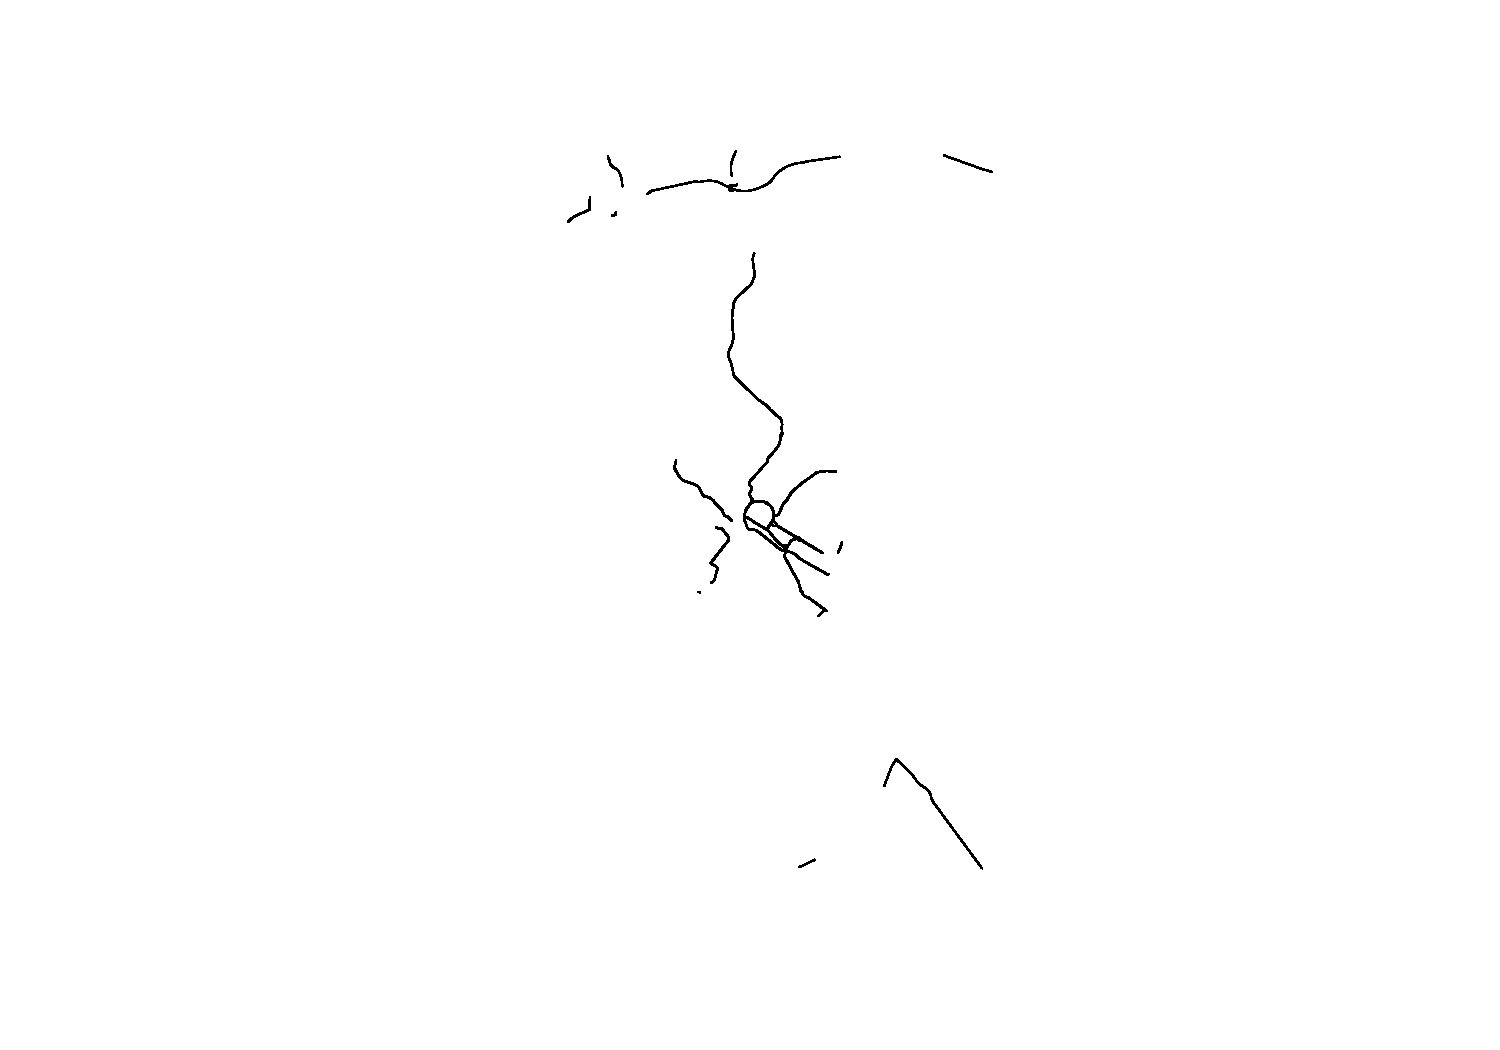
\includegraphics{slides_all2gether_part2_files/figure-beamer/unnamed-chunk-78-1.pdf}

\end{frame}

\begin{frame}[fragile]{Import von Layer \texttt{points}}

\begin{Shaded}
\begin{Highlighting}[]
\NormalTok{datp <-}\StringTok{ }\KeywordTok{st_read}\NormalTok{(}\StringTok{"../data/Amsterdam_highway_primary.osm"}\NormalTok{,}\StringTok{"points"}\NormalTok{)}
\end{Highlighting}
\end{Shaded}

\begin{verbatim}
## Reading layer `points' from data source `D:\Daten\GitHub\geocourse\data\Amsterdam_highway_primary.osm' using driver `OSM'
## Simple feature collection with 800 features and 10 fields
## geometry type:  POINT
## dimension:      XY
## bbox:           xmin: 8.33654 ymin: 49.32801 xmax: 8.626969 ymax: 49.65208
## epsg (SRID):    4326
## proj4string:    +proj=longlat +datum=WGS84 +no_defs
\end{verbatim}

\begin{Shaded}
\begin{Highlighting}[]
\KeywordTok{plot}\NormalTok{(dat}\OperatorTok{$}\NormalTok{geometry,}\DataTypeTok{pch=}\DecValTok{20}\NormalTok{,}\DataTypeTok{col=}\KeywordTok{rgb}\NormalTok{(}\DecValTok{0}\NormalTok{,}\DecValTok{0}\NormalTok{,}\DecValTok{1}\NormalTok{,.}\DecValTok{1}\NormalTok{))}
\end{Highlighting}
\end{Shaded}


\includegraphics{slides_all2gether_part2_files/figure-beamer/unnamed-chunk-79-1.pdf}

\end{frame}

\begin{frame}[fragile]{Mit einem anderen Paket plotten}

\begin{Shaded}
\begin{Highlighting}[]
\KeywordTok{library}\NormalTok{(tmap)}
\KeywordTok{qtm}\NormalTok{(dat}\OperatorTok{$}\NormalTok{geometry)}
\end{Highlighting}
\end{Shaded}

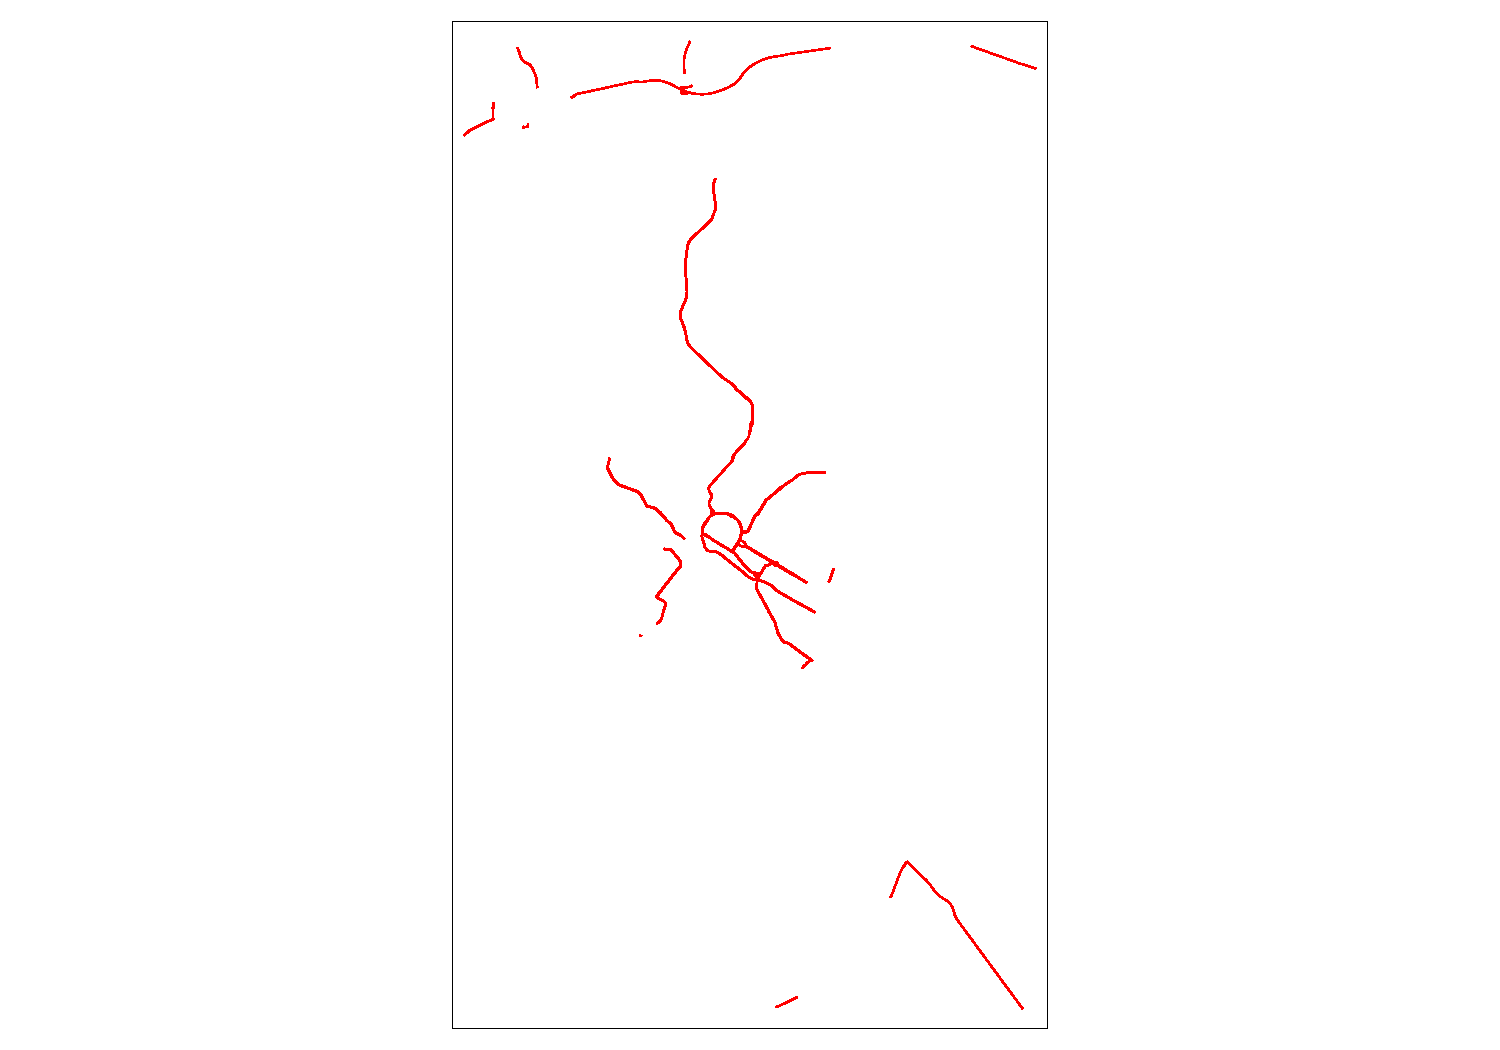
\includegraphics{slides_all2gether_part2_files/figure-beamer/unnamed-chunk-80-1.pdf}

\end{frame}

\begin{frame}[fragile]{}

\begin{Shaded}
\begin{Highlighting}[]
\KeywordTok{st_layers}\NormalTok{(}\StringTok{"../data/ams_centraal.osm"}\NormalTok{)}
\end{Highlighting}
\end{Shaded}

\begin{verbatim}
## Driver: OSM 
## Available layers:
##         layer_name       geometry_type features fields
## 1           points               Point       NA     10
## 2            lines         Line String       NA      9
## 3 multilinestrings   Multi Line String       NA      4
## 4    multipolygons       Multi Polygon       NA     25
## 5  other_relations Geometry Collection       NA      4
\end{verbatim}

\begin{Shaded}
\begin{Highlighting}[]
\NormalTok{datm <-}\StringTok{ }\KeywordTok{st_read}\NormalTok{(}\StringTok{"../data/ams_centraal.osm"}\NormalTok{,}\StringTok{"multipolygons"}\NormalTok{)}
\end{Highlighting}
\end{Shaded}

\begin{verbatim}
## Reading layer `multipolygons' from data source `D:\Daten\GitHub\geocourse\data\ams_centraal.osm' using driver `OSM'
## Simple feature collection with 2796 features and 25 fields
## geometry type:  MULTIPOLYGON
## dimension:      XY
## bbox:           xmin: 4.874776 ymin: 52.36088 xmax: 4.929755 ymax: 52.39393
## epsg (SRID):    4326
## proj4string:    +proj=longlat +datum=WGS84 +no_defs
\end{verbatim}

\begin{Shaded}
\begin{Highlighting}[]
\NormalTok{sp}\OperatorTok{::}\KeywordTok{plot}\NormalTok{(datm}\OperatorTok{$}\NormalTok{geometry)}
\end{Highlighting}
\end{Shaded}

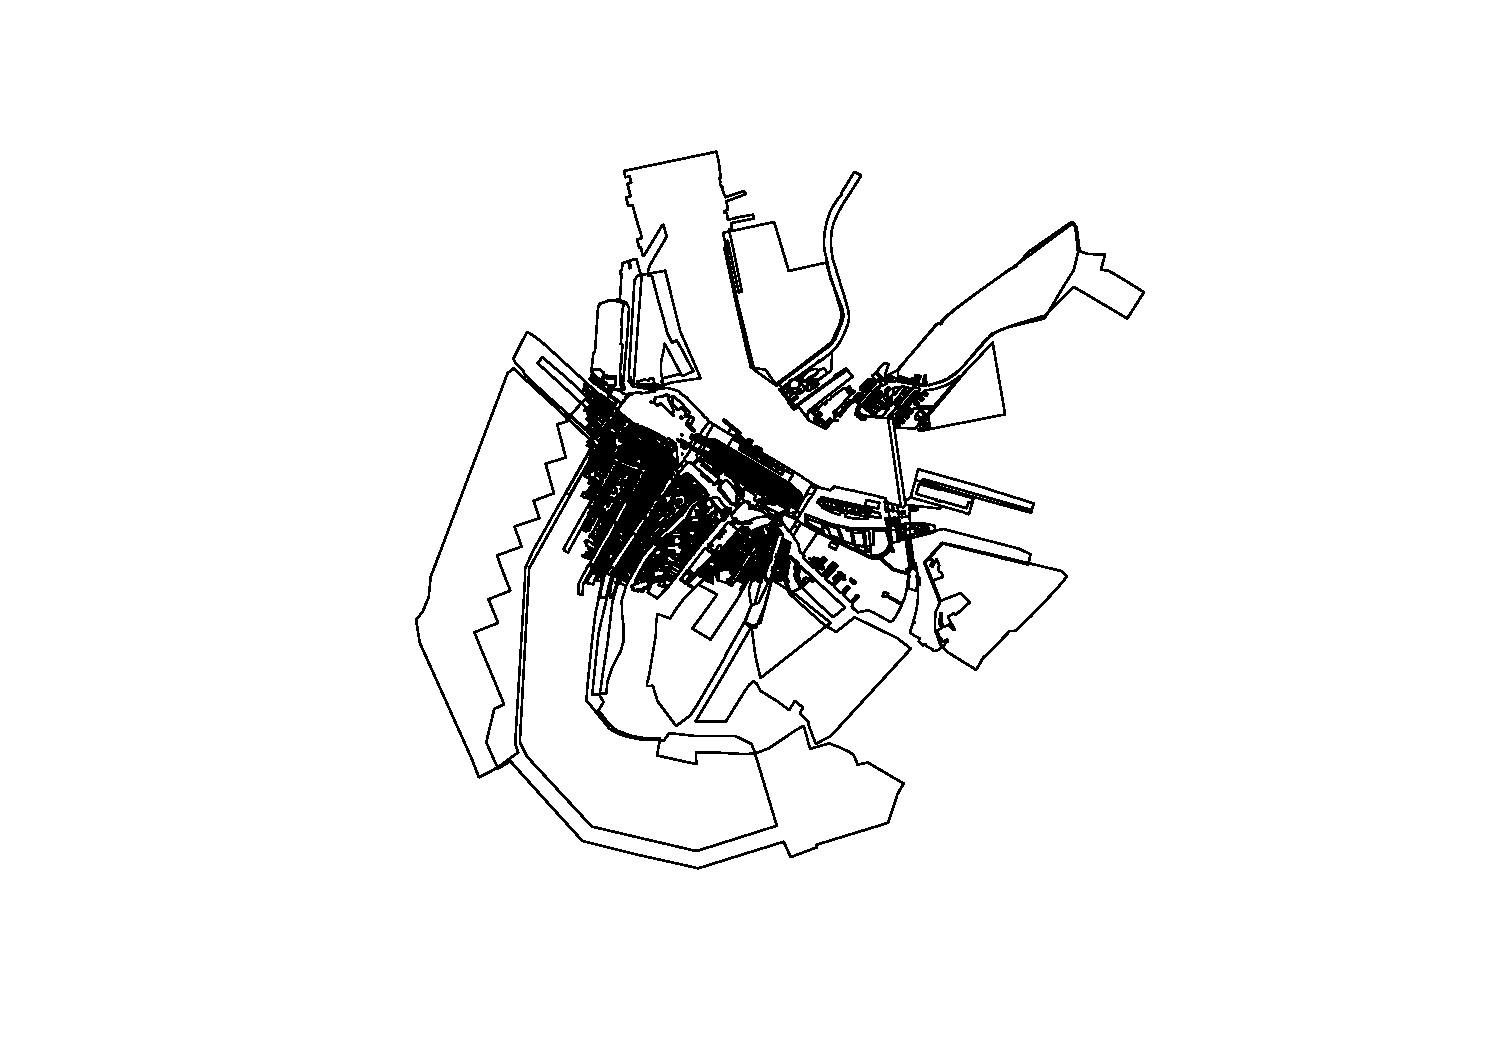
\includegraphics{slides_all2gether_part2_files/figure-beamer/unnamed-chunk-82-1.pdf}

\end{frame}

\begin{frame}{Mehr Beispiele, wie man mit XML Daten umgeht:}

\begin{itemize}
\item
  Deborah Nolan -
  \href{http://www.stat.berkeley.edu/~statcur/Workshop2/Presentations/XML.pdf}{\textbf{Extracting
  data from XML}}
\item
  Duncan Temple Lang -
  \href{http://www.omegahat.net/RSXML/shortIntro.pdf}{\textbf{A Short
  Introduction to the XML package for R}}
\end{itemize}

\begin{block}{Noch mehr Informationen}

\begin{itemize}
\item
  \href{http://www.di.fc.ul.pt/~jpn/r/web/index.html\#parsing-xml}{\textbf{Web
  Daten manipulieren}}
\item
  \href{http://www.w3schools.com/xml/xquery_intro.asp}{\textbf{Tutorial
  zu xquery}}
\item
  \href{http://giventhedata.blogspot.de/2012/06/r-and-web-for-beginners-part-ii-xml-in.html}{\textbf{R
  und das Web (für Anfänger), Teil II: XML und R}}
\item
  Gaston Sanchez -
  \href{http://gastonsanchez.com/Handling_and_Processing_Strings_in_R.pdf}{\textbf{String
  Manipulation}}
\item
  \href{https://www.e-education.psu.edu/geog585/node/738}{\textbf{Nutzung,
  Vor- und Nachteile OSM}}
\item
  \href{http://wiki.openstreetmap.org/wiki/Research}{\textbf{Forschungsprojekte
  im Zusammenhang mit OpenStreetMap}}
\end{itemize}

\end{block}

\end{frame}

\begin{frame}[fragile]{Referenzen}

\begin{Shaded}
\begin{Highlighting}[]
\KeywordTok{citation}\NormalTok{(}\StringTok{"XML"}\NormalTok{)}
\end{Highlighting}
\end{Shaded}

\begin{verbatim}
## 
## To cite package 'XML' in publications use:
## 
##   Duncan Temple Lang and the CRAN Team (2018). XML: Tools for
##   Parsing and Generating XML Within R and S-Plus. R package
##   version 3.98-1.12. https://CRAN.R-project.org/package=XML
## 
## A BibTeX entry for LaTeX users is
## 
##   @Manual{,
##     title = {XML: Tools for Parsing and Generating XML Within R and S-Plus},
##     author = {Duncan Temple Lang and the CRAN Team},
##     year = {2018},
##     note = {R package version 3.98-1.12},
##     url = {https://CRAN.R-project.org/package=XML},
##   }
## 
## ATTENTION: This citation information has been auto-generated from
## the package DESCRIPTION file and may need manual editing, see
## 'help("citation")'.
\end{verbatim}

\end{frame}

\begin{frame}[fragile]{Das neuere Paket}

\begin{Shaded}
\begin{Highlighting}[]
\KeywordTok{citation}\NormalTok{(}\StringTok{"xml2"}\NormalTok{)}
\end{Highlighting}
\end{Shaded}

\begin{verbatim}
## 
## To cite package 'xml2' in publications use:
## 
##   Hadley Wickham, James Hester and Jeroen Ooms (2018). xml2: Parse
##   XML. R package version 1.2.0.
##   https://CRAN.R-project.org/package=xml2
## 
## A BibTeX entry for LaTeX users is
## 
##   @Manual{,
##     title = {xml2: Parse XML},
##     author = {Hadley Wickham and James Hester and Jeroen Ooms},
##     year = {2018},
##     note = {R package version 1.2.0},
##     url = {https://CRAN.R-project.org/package=xml2},
##   }
\end{verbatim}

\end{frame}

\begin{frame}[fragile]{Themen dieses Abschnitts}

\begin{itemize}
\item
  Das R-Paket \texttt{osmdata} mit dem man OSM-Daten herunterladen kann
  und das auf der
  \href{https://wiki.openstreetmap.org/wiki/Overpass_API}{\textbf{Overpass
  API}} beruht.
\item
  Das Paket \texttt{osmplotr}
\end{itemize}

\end{frame}

\begin{frame}{\href{https://github.com/ropensci/osmdata}{Das
\texttt{osmdata} Paket}}


\includegraphics{figure/osmdatatitle.png}

\begin{quote}
Mark Padgham - Import `OpenStreetMap' Data as Simple Features or Spatial
Objects
\end{quote}

\end{frame}

\begin{frame}[fragile]{Das \texttt{osmdata} Paket}

\begin{itemize}
\tightlist
\item
  Mit dem Paket kann man Daten von OpenStreetMap importieren
\item
  Die OSM Daten sind unter
  \href{https://www.openstreetmap.org/copyright}{\textbf{ODbL licence}}
  zu haben
\end{itemize}

\begin{Shaded}
\begin{Highlighting}[]
\KeywordTok{install.packages}\NormalTok{(}\StringTok{"osmdata"}\NormalTok{)}
\end{Highlighting}
\end{Shaded}

\begin{Shaded}
\begin{Highlighting}[]
\KeywordTok{library}\NormalTok{(osmdata)}
\end{Highlighting}
\end{Shaded}

\begin{Shaded}
\begin{Highlighting}[]
\KeywordTok{citation}\NormalTok{(}\StringTok{"osmdata"}\NormalTok{)}
\end{Highlighting}
\end{Shaded}

\end{frame}

\begin{frame}[fragile]{Das Paket \texttt{osmplotr}}

\begin{Shaded}
\begin{Highlighting}[]
\KeywordTok{library}\NormalTok{(}\StringTok{"osmplotr"}\NormalTok{)}
\KeywordTok{library}\NormalTok{(}\StringTok{"osmdata"}\NormalTok{)}
\end{Highlighting}
\end{Shaded}

\end{frame}

\begin{frame}[fragile]{Beispiel Kindergärten in Mannheim}

\begin{Shaded}
\begin{Highlighting}[]
\NormalTok{bbox <-}\StringTok{ }\KeywordTok{getbb}\NormalTok{(}\StringTok{"Mannheim"}\NormalTok{)}
\NormalTok{dat_osm <-}\StringTok{ }\KeywordTok{extract_osm_objects}\NormalTok{(}\DataTypeTok{key=}\StringTok{'building'}\NormalTok{, }
                              \DataTypeTok{value=}\StringTok{"kindergarten"}\NormalTok{,}
                              \DataTypeTok{bbox=}\NormalTok{bbox)}
\end{Highlighting}
\end{Shaded}

\end{frame}

\begin{frame}[fragile]{Einen Rahmen definieren um Daten zu bekommen}

\begin{itemize}
\tightlist
\item
  Der Rahmen kann entweder erstellt werden, indem die Koordinaten
  angegeben werden:
\end{itemize}

\begin{Shaded}
\begin{Highlighting}[]
\NormalTok{q <-}\StringTok{ }\KeywordTok{opq}\NormalTok{(}\DataTypeTok{bbox =} \KeywordTok{c}\NormalTok{(}\FloatTok{52.3}\NormalTok{, }\FloatTok{4.7}\NormalTok{, }\FloatTok{52.4}\NormalTok{, }\FloatTok{5.1}\NormalTok{))}
\end{Highlighting}
\end{Shaded}

\begin{itemize}
\tightlist
\item
  oder indem man den Befehl \texttt{getbb} verwendet:
\end{itemize}

\begin{Shaded}
\begin{Highlighting}[]
\NormalTok{bb <-}\StringTok{ }\KeywordTok{getbb}\NormalTok{(}\StringTok{'Ladenburg'}\NormalTok{)}
\end{Highlighting}
\end{Shaded}

\begin{itemize}
\item
  In \texttt{bb} sind nun vier Werte gespeichert, die den Rahmen
  definieren
\item
  Befehl \texttt{opq} - eine Overpass Anfrage erstellen
\end{itemize}

\begin{Shaded}
\begin{Highlighting}[]
\NormalTok{q <-}\StringTok{ }\KeywordTok{opq}\NormalTok{(}\DataTypeTok{bbox =}\NormalTok{ bb)}
\end{Highlighting}
\end{Shaded}

\end{frame}

\begin{frame}[fragile]{Die Grenze von Mannheim}

\begin{itemize}
\tightlist
\item
  Erst mit dem Argument \texttt{format\_out=polygon} Befehl
  \texttt{getbb} erhält man das Polygon:
\end{itemize}

\begin{Shaded}
\begin{Highlighting}[]
\NormalTok{bb_poly <-}\StringTok{ }\KeywordTok{getbb}\NormalTok{(}\DataTypeTok{place_name =} \StringTok{"Ladenburg"}\NormalTok{, }
                 \DataTypeTok{format_out =} \StringTok{"polygon"}\NormalTok{)}
\end{Highlighting}
\end{Shaded}

\begin{itemize}
\tightlist
\item
  Das Ergebnis ist sind zwei Vektoren mit den Longitude und Latitude
  Koordinaten.
\end{itemize}

\begin{verbatim}
##          [,1]     [,2]
## [1,] 8.569720 49.49107
## [2,] 8.569858 49.49101
## [3,] 8.569999 49.49096
## [4,] 8.570342 49.49085
\end{verbatim}

\end{frame}

\begin{frame}[fragile]{Das Paket für simple feature (\texttt{sf})}

\begin{quote}
Simple Features for R
\end{quote}

\begin{itemize}
\tightlist
\item
  Das Paket \texttt{sf} ist ein Paket um geometrische Operationen
  durchzuführen.
\end{itemize}

\begin{Shaded}
\begin{Highlighting}[]
\KeywordTok{library}\NormalTok{(sf)}
\end{Highlighting}
\end{Shaded}

\begin{itemize}
\tightlist
\item
  \href{https://cran.r-project.org/web/packages/sf/vignettes/sf3.html}{\textbf{Vignette
  für das Paket \texttt{sf}}}
\end{itemize}

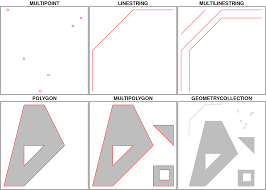
\includegraphics{figure/rsimplefeatures.png}

\end{frame}

\begin{frame}[fragile]{Die Funktion \texttt{st\_linestring}}

\begin{quote}
Create simple feature from a numeric vector, matrix or list
\end{quote}

\begin{Shaded}
\begin{Highlighting}[]
\KeywordTok{library}\NormalTok{(sf)}
\NormalTok{ls <-}\StringTok{ }\KeywordTok{st_linestring}\NormalTok{(bb_poly)}
\NormalTok{sfc <-}\StringTok{ }\KeywordTok{st_sfc}\NormalTok{(ls)}
\end{Highlighting}
\end{Shaded}

\end{frame}

\begin{frame}[fragile]{Den \texttt{linestring} plotten}

\begin{Shaded}
\begin{Highlighting}[]
\KeywordTok{library}\NormalTok{(tmap)}
\KeywordTok{qtm}\NormalTok{(sfc)}
\end{Highlighting}
\end{Shaded}

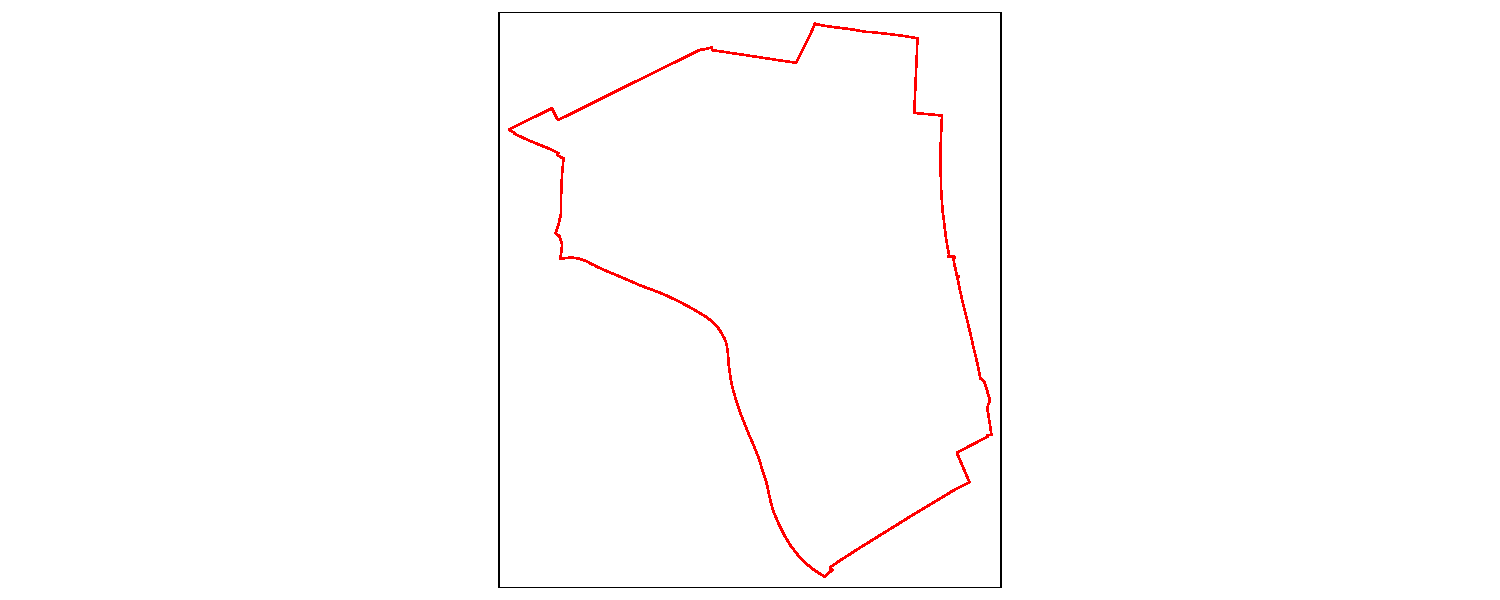
\includegraphics{slides_all2gether_part2_files/figure-beamer/unnamed-chunk-101-1.pdf}

\end{frame}

\begin{frame}[fragile]{Einrichtungen (amenity)}

\begin{block}{\href{https://wiki.openstreetmap.org/wiki/Map_Features}{\textbf{OSM
map features}}}

\begin{itemize}
\item
  Alle benannten Objekte findet man, wenn man OSM map features in eine
  Suchmaschine eingibt.
\item
  Achtung, wenn man bspw. alle Objekte mit dem Schlüssel
  \texttt{amenity} für eine Stadt heraussucht, bekommt man einen recht
  großen Datensatz
\end{itemize}

\begin{Shaded}
\begin{Highlighting}[]
\NormalTok{q <-}\StringTok{ }\KeywordTok{add_osm_feature}\NormalTok{ (q, }\DataTypeTok{key =} \StringTok{'amenity'}\NormalTok{)}
\KeywordTok{osmdata_xml}\NormalTok{(q, }\StringTok{'../data/Ladenburg_amenity.osm'}\NormalTok{)}
\end{Highlighting}
\end{Shaded}

\end{block}

\end{frame}

\begin{frame}{Was dahinter steckt}

\end{frame}

\begin{frame}[fragile]{Die Funktion \texttt{osmdata\_sf}}

\begin{itemize}
\tightlist
\item
  Die Funktion \texttt{osmdata\_sf} gibt ein \texttt{osmdata} ObjeKt im
  \texttt{sf} Format.
\end{itemize}

\begin{Shaded}
\begin{Highlighting}[]
\KeywordTok{library}\NormalTok{(magrittr)}
\NormalTok{dat1 <-}\StringTok{ }\KeywordTok{opq}\NormalTok{(}\DataTypeTok{bbox =} \StringTok{'Ladenburg'}\NormalTok{) }\OperatorTok
\StringTok{    }\KeywordTok{add_osm_feature}\NormalTok{(}\DataTypeTok{key =} \StringTok{'shop'}\NormalTok{, }\DataTypeTok{value =} \StringTok{'bakery'}\NormalTok{) }\OperatorTok
\StringTok{    }\KeywordTok{osmdata_sf}\NormalTok{ ()}
\end{Highlighting}
\end{Shaded}

\begin{Shaded}
\begin{Highlighting}[]
\KeywordTok{unlist}\NormalTok{(}\KeywordTok{lapply}\NormalTok{(dat1,nrow))}
\end{Highlighting}
\end{Shaded}

\begin{verbatim}
##        osm_points         osm_lines      osm_polygons    osm_multilines 
##                16                 0                 0                 0 
## osm_multipolygons 
##                 0
\end{verbatim}

\end{frame}

\begin{frame}[fragile]{Alles in eine Karte plotten}

\begin{block}{\href{https://cran.r-project.org/web/packages/tmap/vignettes/tmap-getstarted.html}{**Der
Start mit dem Paket \texttt{tmap}}}

\begin{Shaded}
\begin{Highlighting}[]
\KeywordTok{library}\NormalTok{(tmap)}
\KeywordTok{tm_shape}\NormalTok{(sfc) }
\KeywordTok{tm_bubbles}\NormalTok{(dat, }\DataTypeTok{size=}\DecValTok{2}\NormalTok{)}
\end{Highlighting}
\end{Shaded}

\end{block}

\end{frame}

\begin{frame}[fragile]{Beispiel Fahrradparkplätze}

\begin{itemize}
\tightlist
\item
  \href{https://wiki.openstreetmap.org/wiki/Map_Features\#Highway}{\textbf{OSM
  map features}}
\end{itemize}

\begin{Shaded}
\begin{Highlighting}[]
\NormalTok{q <-}\StringTok{ }\KeywordTok{add_osm_feature}\NormalTok{ (q, }\DataTypeTok{key =} \StringTok{'amenity'}\NormalTok{,}\DataTypeTok{value =} \StringTok{"bicycle_parking"}\NormalTok{)}
\KeywordTok{osmdata_xml}\NormalTok{(q, }\StringTok{'../data/Amsterdam_amenity_bicycle_parking.osm'}\NormalTok{)}
\end{Highlighting}
\end{Shaded}

\begin{Shaded}
\begin{Highlighting}[]
\NormalTok{dat <-}\StringTok{ }\NormalTok{sf}\OperatorTok{::}\KeywordTok{st_read}\NormalTok{ (}\StringTok{'../data/Amsterdam_amenity_bicycle_parking.osm'}\NormalTok{, }
                    \DataTypeTok{layer =} \StringTok{'points'}\NormalTok{, }
                    \DataTypeTok{quiet =} \OtherTok{TRUE}\NormalTok{)}
\end{Highlighting}
\end{Shaded}

\end{frame}

\begin{frame}[fragile]{Die Daten plotten}

\begin{Shaded}
\begin{Highlighting}[]
\KeywordTok{library}\NormalTok{(tmap)}
\KeywordTok{qtm}\NormalTok{(dat)}
\end{Highlighting}
\end{Shaded}

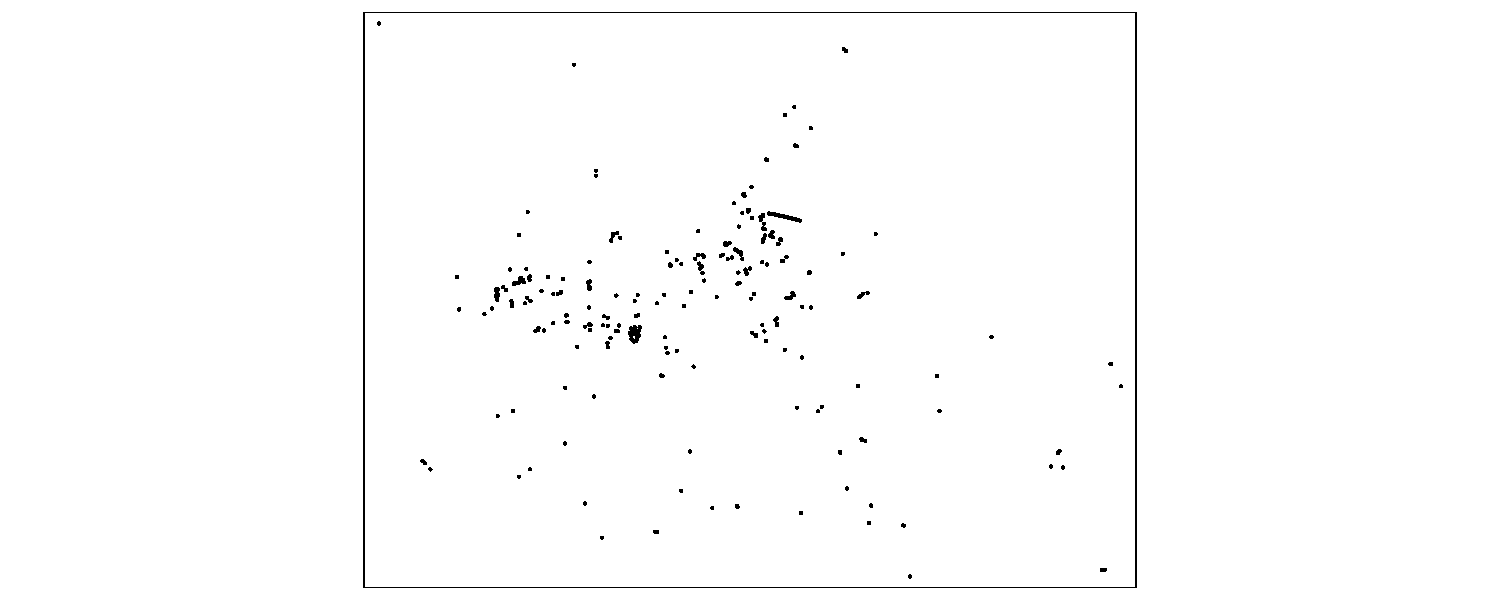
\includegraphics{slides_all2gether_part2_files/figure-beamer/unnamed-chunk-109-1.pdf}

\end{frame}

\begin{frame}[fragile]{Sehen was dahinter steckt}

\begin{Shaded}
\begin{Highlighting}[]
\NormalTok{dat <-}\StringTok{ }\NormalTok{sf}\OperatorTok{::}\KeywordTok{st_read}\NormalTok{ (}\StringTok{'../data/Amsterdam_amenity.osm'}\NormalTok{, }
                    \DataTypeTok{layer =} \StringTok{'points'}\NormalTok{, }
                    \DataTypeTok{quiet =} \OtherTok{TRUE}\NormalTok{)}
\end{Highlighting}
\end{Shaded}

\begin{Shaded}
\begin{Highlighting}[]
\KeywordTok{nrow}\NormalTok{(dat)}
\KeywordTok{names}\NormalTok{(dat)}
\end{Highlighting}
\end{Shaded}

\end{frame}

\begin{frame}[fragile]{Bar`s in Mannheim}

\begin{Shaded}
\begin{Highlighting}[]
\NormalTok{?add_osm_feature}
\end{Highlighting}
\end{Shaded}

\begin{Shaded}
\begin{Highlighting}[]
\NormalTok{q <-}\StringTok{ }\KeywordTok{opq}\NormalTok{ (}\DataTypeTok{bbox =} \StringTok{'Mannheim'}\NormalTok{)}
\NormalTok{q <-}\StringTok{ }\KeywordTok{add_osm_feature}\NormalTok{ (q, }\DataTypeTok{key =}\StringTok{"amenity"}\NormalTok{,}\DataTypeTok{value =} \StringTok{'bar'}\NormalTok{) }
\KeywordTok{osmdata_xml}\NormalTok{ (q, }\StringTok{'data/Mannheim_bar.osm'}\NormalTok{)}
\end{Highlighting}
\end{Shaded}

\begin{Shaded}
\begin{Highlighting}[]
\NormalTok{dat_bar <-}\StringTok{ }\NormalTok{sf}\OperatorTok{::}\KeywordTok{st_read}\NormalTok{ (}\StringTok{'../data/Mannheim_bar.osm'}\NormalTok{, }
                        \DataTypeTok{layer =} \StringTok{'points'}\NormalTok{, }\DataTypeTok{quiet =} \OtherTok{TRUE}\NormalTok{)}
\end{Highlighting}
\end{Shaded}

\end{frame}

\begin{frame}[fragile]{Bus stations in Amsterdam}

\begin{Shaded}
\begin{Highlighting}[]
\NormalTok{q <-}\StringTok{ }\KeywordTok{opq}\NormalTok{ (}\DataTypeTok{bbox =} \StringTok{'Amsterdam'}\NormalTok{)}
\NormalTok{q <-}\StringTok{ }\KeywordTok{add_osm_feature}\NormalTok{ (q, }\DataTypeTok{key =}\StringTok{"amenity"}\NormalTok{,}
                      \DataTypeTok{value =} \StringTok{'bus_station'}\NormalTok{) }
\KeywordTok{osmdata_xml}\NormalTok{ (q, }\StringTok{'data/Amsterdam_bus_station.osm'}\NormalTok{)}
\end{Highlighting}
\end{Shaded}

\begin{Shaded}
\begin{Highlighting}[]
\NormalTok{dat_bus <-}\StringTok{ }\NormalTok{sf}\OperatorTok{::}\KeywordTok{st_read}\NormalTok{ (}\StringTok{'../data/Amsterdam_bus_station.osm'}\NormalTok{, }
                        \DataTypeTok{layer =} \StringTok{'points'}\NormalTok{, }\DataTypeTok{quiet =} \OtherTok{TRUE}\NormalTok{)}
\KeywordTok{nrow}\NormalTok{(dat_bus)}
\end{Highlighting}
\end{Shaded}

\begin{Shaded}
\begin{Highlighting}[]
\NormalTok{?sf}\OperatorTok{::}\NormalTok{st_read}
\end{Highlighting}
\end{Shaded}

\end{frame}

\begin{frame}[fragile]{An alternative}

\begin{itemize}
\tightlist
\item
  \href{https://github.com/ropensci/osmdata/blob/master/vignettes/osmdata.Rmd}{Main
  vignette \texttt{osmdata}}
\item
  \href{https://cran.r-project.org/web/packages/osmdata/vignettes/osm-sf-translation.html}{OpenStreetMap
  Data Structure}
\end{itemize}

\begin{Shaded}
\begin{Highlighting}[]
\NormalTok{q <-}\StringTok{ }\KeywordTok{opq}\NormalTok{ (}\DataTypeTok{bbox =} \StringTok{'Amsterdam'}\NormalTok{)}
\NormalTok{q <-}\StringTok{ }\KeywordTok{add_osm_feature}\NormalTok{ (q, }\DataTypeTok{key =}\StringTok{"public_transport"}\NormalTok{,}
                      \DataTypeTok{value =} \StringTok{'station'}\NormalTok{) }
\KeywordTok{osmdata_xml}\NormalTok{ (q, }\StringTok{'../data/Amsterdam_bus_pubtrans.osm'}\NormalTok{)}
\end{Highlighting}
\end{Shaded}

\begin{Shaded}
\begin{Highlighting}[]
\NormalTok{dat_bus <-}\StringTok{ }\NormalTok{sf}\OperatorTok{::}\KeywordTok{st_read}\NormalTok{ (}\StringTok{'../data/Amsterdam_bus_pubtrans.osm'}\NormalTok{, }
                        \DataTypeTok{layer =} \StringTok{'points'}\NormalTok{, }\DataTypeTok{quiet =} \OtherTok{TRUE}\NormalTok{)}
\KeywordTok{nrow}\NormalTok{(dat_bus)}
\end{Highlighting}
\end{Shaded}

\end{frame}

\begin{frame}[fragile]{Further information about public transport}

\begin{block}{Stop area}

\begin{Shaded}
\begin{Highlighting}[]
\NormalTok{dat3 <-}\StringTok{ }\KeywordTok{opq}\NormalTok{(}\DataTypeTok{bbox =} \StringTok{'Amsterdam'}\NormalTok{) }\OperatorTok
\StringTok{    }\KeywordTok{add_osm_feature}\NormalTok{(}\DataTypeTok{key =} \StringTok{'railway'}\NormalTok{, }
                    \DataTypeTok{value =} \StringTok{'tram_stop'}\NormalTok{) }\OperatorTok
\StringTok{    }\KeywordTok{osmdata_sf}\NormalTok{ ()}
\end{Highlighting}
\end{Shaded}

\begin{Shaded}
\begin{Highlighting}[]
\NormalTok{dat3}\OperatorTok{$}\NormalTok{osm_points}\OperatorTok{$}\NormalTok{geometry}
\end{Highlighting}
\end{Shaded}

\end{block}

\end{frame}

\begin{frame}[fragile]{Plotting the result}

\begin{Shaded}
\begin{Highlighting}[]
\CommentTok{# install.packages("osmplotr")}
\KeywordTok{library}\NormalTok{(}\StringTok{"osmplotr"}\NormalTok{)}
\NormalTok{bbox <-}\StringTok{ }\KeywordTok{getbb}\NormalTok{(}\StringTok{"Amsterdam"}\NormalTok{)}
\NormalTok{dat_pa <-}\StringTok{ }\KeywordTok{extract_osm_objects}\NormalTok{(}\DataTypeTok{key=}\StringTok{'highway'}\NormalTok{, }
                              \DataTypeTok{value=}\StringTok{"primary"}\NormalTok{,}
                              \DataTypeTok{bbox=}\NormalTok{bbox)}
\NormalTok{dat_sa <-}\StringTok{ }\KeywordTok{extract_osm_objects}\NormalTok{(}\DataTypeTok{key=}\StringTok{'highway'}\NormalTok{, }
                              \DataTypeTok{value=}\StringTok{"secondary"}\NormalTok{,}
                              \DataTypeTok{bbox=}\NormalTok{bbox)}
\NormalTok{dat_ta <-}\StringTok{ }\KeywordTok{extract_osm_objects}\NormalTok{(}\DataTypeTok{key=}\StringTok{'highway'}\NormalTok{, }
                              \DataTypeTok{value=}\StringTok{"tertiary"}\NormalTok{,}
                              \DataTypeTok{bbox=}\NormalTok{bbox)}
\end{Highlighting}
\end{Shaded}

\begin{Shaded}
\begin{Highlighting}[]
\NormalTok{map <-}\StringTok{ }\KeywordTok{osm_basemap}\NormalTok{(}\DataTypeTok{bbox =}\NormalTok{ bbox, }\DataTypeTok{bg =} \KeywordTok{c}\NormalTok{(}\StringTok{"#F5F5DC"}\NormalTok{))}
\NormalTok{map <-}\StringTok{ }\KeywordTok{add_osm_objects}\NormalTok{(map, dat_pa, }\DataTypeTok{col =} \KeywordTok{c}\NormalTok{(}\StringTok{"#00008B"}\NormalTok{))}
\NormalTok{map <-}\StringTok{ }\KeywordTok{add_osm_objects}\NormalTok{(map, dat_sa, }\DataTypeTok{col =} \StringTok{"green"}\NormalTok{)}
\NormalTok{map <-}\StringTok{ }\KeywordTok{add_osm_objects}\NormalTok{(map, dat_ta, }\DataTypeTok{col =} \StringTok{"lightblue"}\NormalTok{)}
\NormalTok{map <-}\StringTok{ }\KeywordTok{add_osm_objects}\NormalTok{(map, dat3}\OperatorTok{$}\NormalTok{osm_points, }\DataTypeTok{col =} \KeywordTok{c}\NormalTok{(}\StringTok{"red"}\NormalTok{))}
\KeywordTok{print_osm_map}\NormalTok{(map)}
\end{Highlighting}
\end{Shaded}

\end{frame}

\begin{frame}[fragile]{Get an overview of the available features}

\begin{Shaded}
\begin{Highlighting}[]
\NormalTok{features <-}\StringTok{ }\KeywordTok{available_features}\NormalTok{()}
\KeywordTok{head}\NormalTok{(features,}\DataTypeTok{n=}\DecValTok{20}\NormalTok{)}
\end{Highlighting}
\end{Shaded}

\begin{verbatim}
##  [1] "4wd only"                "abandoned"              
##  [3] "abutters"                "access"                 
##  [5] "addr"                    "addr:city"              
##  [7] "addr:conscriptionnumber" "addr:country"           
##  [9] "addr:district"           "addr:flats"             
## [11] "addr:full"               "addr:hamlet"            
## [13] "addr:housename"          "addr:housenumber"       
## [15] "addr:inclusion"          "addr:interpolation"     
## [17] "addr:place"              "addr:postcode"          
## [19] "addr:province"           "addr:state"
\end{verbatim}

\end{frame}

\begin{frame}[fragile]{\href{https://github.com/ropensci/osmdata/issues/126}{Changing
the API}}

\begin{Shaded}
\begin{Highlighting}[]
\NormalTok{api_list <-}\StringTok{ }\KeywordTok{c}\NormalTok{(}\StringTok{'http://overpass-api.de/api/interpreter'}\NormalTok{,}
              \StringTok{'https://lz4.overpass-api.de/api/interpreter'}\NormalTok{,}
              \StringTok{'https://z.overpass-api.de/api/interpreter'}\NormalTok{,}
              \StringTok{'https://overpass.kumi.systems/api/interpreter'}\NormalTok{)}

\NormalTok{api_to_use <-}\StringTok{ }\KeywordTok{sample}\NormalTok{(}\DecValTok{1}\OperatorTok{:}\KeywordTok{length}\NormalTok{(api_list), }\DecValTok{1}\NormalTok{)}

\KeywordTok{set_overpass_url}\NormalTok{(api_list[api_to_use]) }
\end{Highlighting}
\end{Shaded}

\end{frame}

\begin{frame}[fragile]{Die wichtigsten Funktionen im Paket
\texttt{osmdata}}

\begin{Shaded}
\begin{Highlighting}[]
\CommentTok{# https://rdrr.io/cran/osmdata/man/osmdata_sp.html}
\NormalTok{?osmdata_sp}
\end{Highlighting}
\end{Shaded}

\end{frame}

\begin{frame}[fragile]{Links}

\begin{itemize}
\item
  \href{https://github.com/ropensci/osmdata}{Github repo of the
  \texttt{osmdata} package}
\item
  \href{https://cran.r-project.org/web/packages/osmdata/vignettes/osmdata.html}{Vignette
  for the package \texttt{osmdata}} on
  \href{https://github.com/ropensci/osmdata/blob/master/vignettes/osmdata.Rmd}{github}
\item
  \href{https://ropensci.github.io/osmdata/}{osmdata Homepage}
\item
  \href{http://overpass-api.de/query_form.html}{Overpass API - query
  form}
\item
  \href{https://wiki.openstreetmap.org/wiki/DE:Overpass_API/Language_Guide}{Overpass
  API/Language Guide}
\item
  \href{https://wiki.openstreetmap.org/wiki/DE:Overpass_turbo}{Overpass
  Turbo} 
\item
  \href{https://ropensci.org/tutorials/osmplotr_tutorial/}{**\texttt{osmplotr}
  tutorial}
\item
  \href{https://bookdown.org/robinlovelace/geocompr/}{\textbf{Geocomputation
  with R}}
\item
  \href{https://www.theoj.org/joss-papers/joss.00305/10.21105.joss.00305.pdf}{\textbf{osmar
  - JOS}}
\end{itemize}

\end{frame}

\begin{frame}[fragile]{Beispiel zu Campingplätzen}

\begin{itemize}
\tightlist
\item
  Die Daten stammen von:
\end{itemize}

\url{http://www.openstreetmap.de/}

\begin{itemize}
\tightlist
\item
  Dabei wird die Overpass API genutzt:
\end{itemize}

\url{http://wiki.openstreetmap.org/wiki/Overpass_API}

\begin{Shaded}
\begin{Highlighting}[]
\NormalTok{url <-}\StringTok{ "https://raw.githubusercontent.com/Japhilko/}
\StringTok{GeoData/master/2015/data/CampSites_Germany.csv"}
\end{Highlighting}
\end{Shaded}

\begin{Shaded}
\begin{Highlighting}[]
\NormalTok{CampSites <-}\StringTok{ }\KeywordTok{read.csv}\NormalTok{(url)}
\end{Highlighting}
\end{Shaded}

\end{frame}

\begin{frame}{Überblick über Daten zu Campingplätzen}

\begin{longtable}[]{@{}rlll@{}}
\toprule
X & name & tourism & website\tabularnewline
\midrule
\endhead
1 & Campingplatz Winkelbachtal & camp\_site &
\url{http://www.gruibingen.de/campingplatz.html}\tabularnewline
2 & Radler-Zeltplatz & camp\_site & NA\tabularnewline
3 & Campingplatz des Naturfreundehauses & camp\_site & NA\tabularnewline
4 & Campingplatz Am Aichstruter Stausee & camp\_site & NA\tabularnewline
5 & NA & camp\_site & NA\tabularnewline
6 & Kandern & camp\_site & NA\tabularnewline
7 & Campingplatz Baiersbronn-Obertal & camp\_site & NA\tabularnewline
8 & Campingplatz Schwabenmühle & camp\_site & NA\tabularnewline
\bottomrule
\end{longtable}

\end{frame}

\begin{frame}[fragile]{Notwendige Pakete}

\href{https://cran.r-project.org/web/packages/magrittr/index.html}{magrittr}
- für den Pipe Operator in R:

\begin{Shaded}
\begin{Highlighting}[]
\KeywordTok{library}\NormalTok{(}\StringTok{"magrittr"}\NormalTok{)}
\end{Highlighting}
\end{Shaded}

\href{https://rstudio.github.io/leaflet/}{leaflet} - um interaktive
Karten mit der JavaScript Bibliothek `Leaflet' zu erzeugen

\begin{Shaded}
\begin{Highlighting}[]
\KeywordTok{library}\NormalTok{(}\StringTok{"leaflet"}\NormalTok{)}
\end{Highlighting}
\end{Shaded}

\end{frame}

\begin{frame}[fragile]{Eine erste interaktive Karte}

\begin{Shaded}
\begin{Highlighting}[]
\KeywordTok{leaflet}\NormalTok{()}\OperatorTok
\StringTok{  }\KeywordTok{addTiles}\NormalTok{()}
\end{Highlighting}
\end{Shaded}

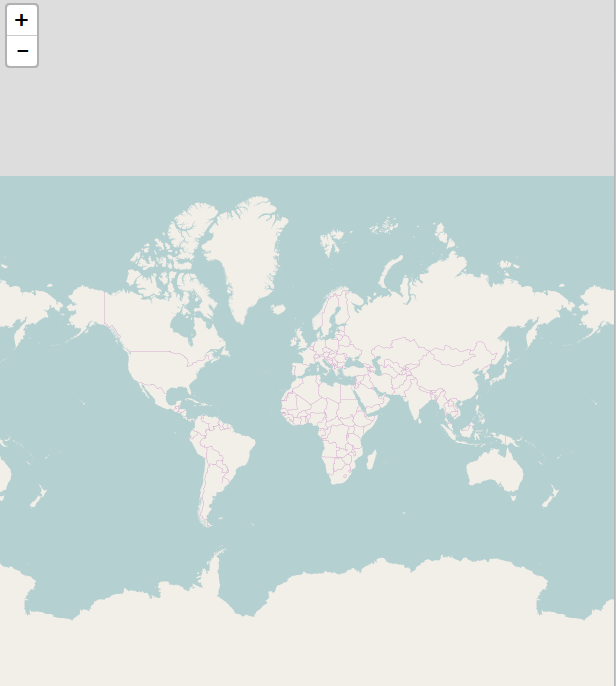
\includegraphics{figure/FirstLeaflet.PNG}

\end{frame}

\begin{frame}[fragile]{Auf eine Stadt zoomen}

\begin{Shaded}
\begin{Highlighting}[]
\KeywordTok{leaflet}\NormalTok{() }\OperatorTok
\StringTok{  }\KeywordTok{addTiles}\NormalTok{() }\OperatorTok
\StringTok{  }\KeywordTok{addMarkers}\NormalTok{(}\DataTypeTok{lng=}\FloatTok{8.456597}\NormalTok{, }\DataTypeTok{lat=}\FloatTok{49.48738}\NormalTok{,}
             \DataTypeTok{popup=}\StringTok{"Wo wir sind"}\NormalTok{)}
\end{Highlighting}
\end{Shaded}

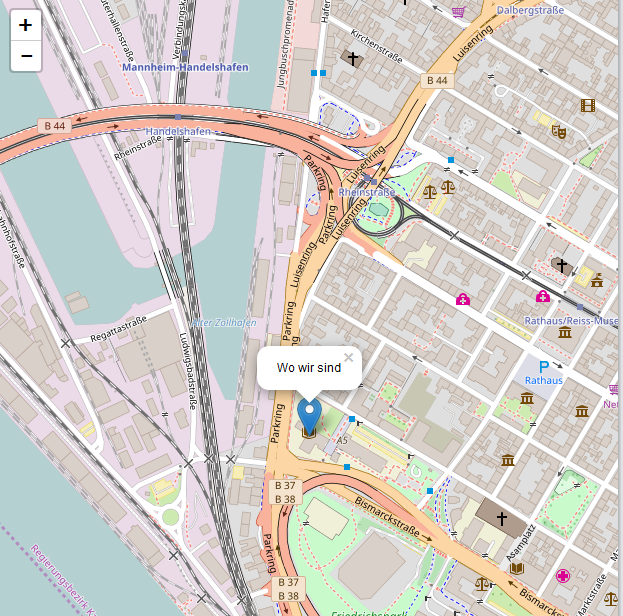
\includegraphics{figure/leafletMZESMA.PNG}

\end{frame}

\begin{frame}[fragile]{Eine interaktive Karte}

\begin{Shaded}
\begin{Highlighting}[]
\NormalTok{m <-}\StringTok{ }\KeywordTok{leaflet}\NormalTok{() }\OperatorTok
\StringTok{  }\KeywordTok{addTiles}\NormalTok{() }\OperatorTok\StringTok{  }
\StringTok{  }\KeywordTok{addMarkers}\NormalTok{(}\DataTypeTok{lng=}\NormalTok{CampSites}\OperatorTok{$}\NormalTok{lon, }
             \DataTypeTok{lat=}\NormalTok{CampSites}\OperatorTok{$}\NormalTok{lat, }
             \DataTypeTok{popup=}\NormalTok{CampSites}\OperatorTok{$}\NormalTok{name)}
\NormalTok{m}
\end{Highlighting}
\end{Shaded}

\end{frame}

\begin{frame}[fragile]{\href{https://rstudio.github.io/leaflet/basemaps.html}{Stamen
als Hintergrundkarte}}

\begin{Shaded}
\begin{Highlighting}[]
\NormalTok{m }\OperatorTok\StringTok{ }\KeywordTok{addProviderTiles}\NormalTok{(}\StringTok{"Stamen.Toner"}\NormalTok{)}
\end{Highlighting}
\end{Shaded}

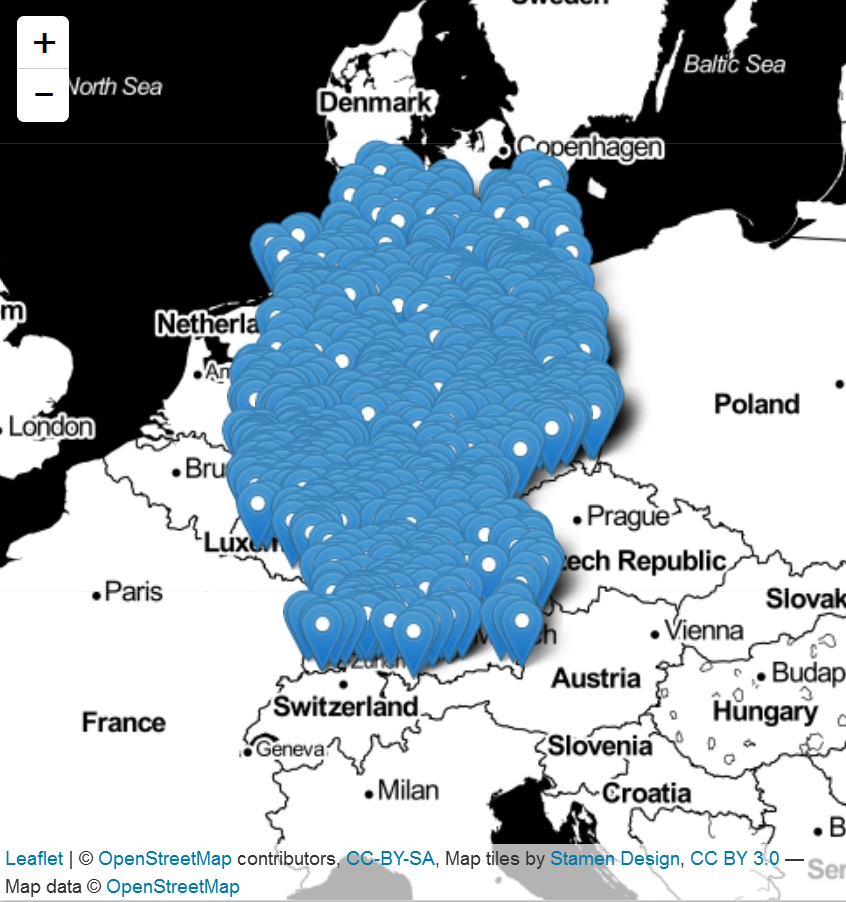
\includegraphics{figure/InteractiveStamen.PNG}

\end{frame}

\begin{frame}[fragile]{CartoDB als Hintergrund}

\begin{Shaded}
\begin{Highlighting}[]
\NormalTok{m }\OperatorTok\StringTok{ }\KeywordTok{addProviderTiles}\NormalTok{(}\StringTok{"CartoDB.Positron"}\NormalTok{)}
\end{Highlighting}
\end{Shaded}

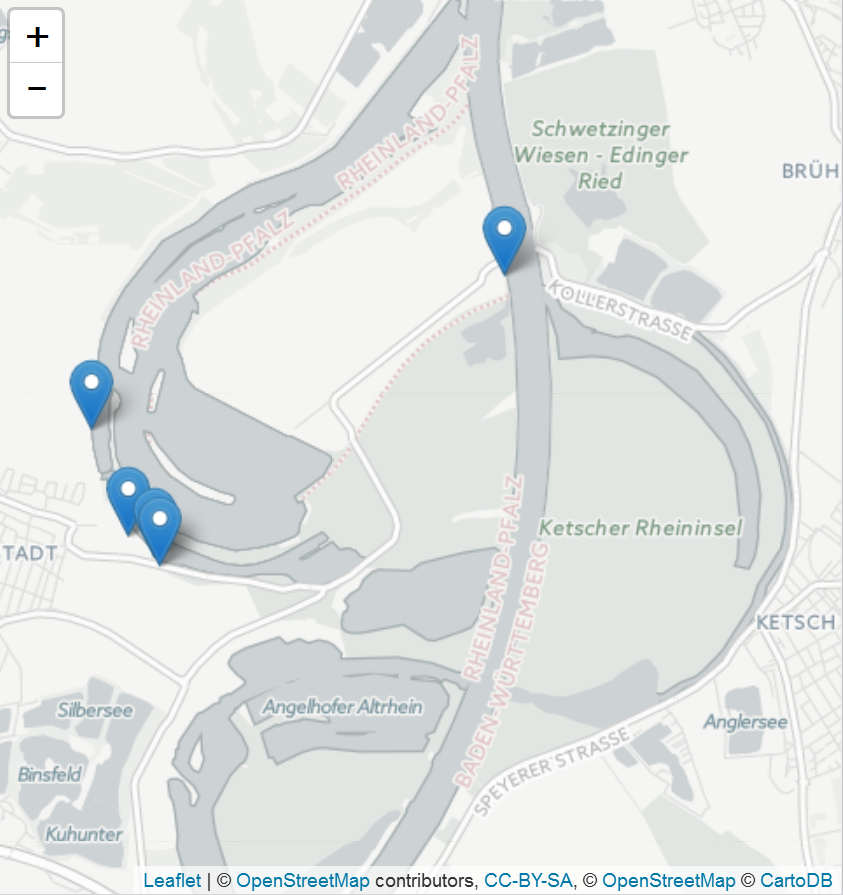
\includegraphics{figure/CartoDBInteractive.PNG}

\begin{itemize}
\item
  \href{https://carto.com/attribution}{CartoDB}
\item
  \href{https://www.mapbox.com/help/how-web-maps-work/}{Info zu Map
  Tiles}
\end{itemize}

\end{frame}

\begin{frame}[fragile]{\href{http://leaflet-extras.github.io/leaflet-providers/preview/index.html}{Mehr
Hintergründe}}

\begin{Shaded}
\begin{Highlighting}[]
\NormalTok{m }\OperatorTok\StringTok{ }\KeywordTok{addProviderTiles}\NormalTok{(}\StringTok{"NASAGIBS.ViirsEarthAtNight2012"}\NormalTok{)}
\end{Highlighting}
\end{Shaded}

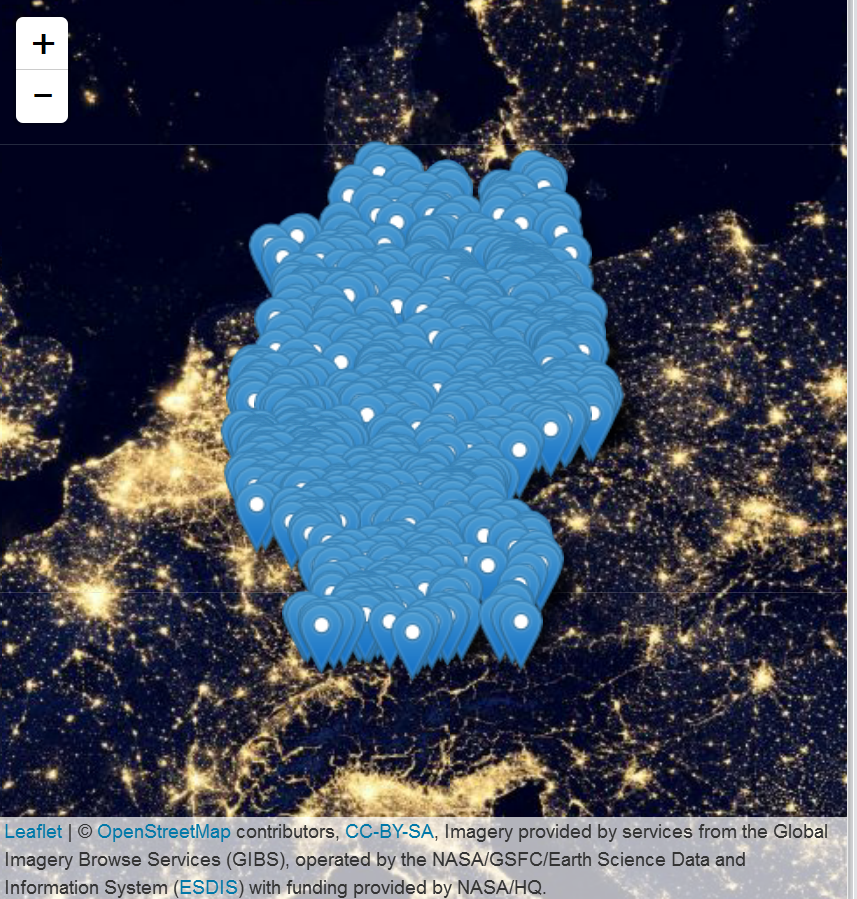
\includegraphics{figure/LightsInteractive.PNG}

\end{frame}

\begin{frame}[fragile]{Mehr Informationen hinzufügen}

\begin{Shaded}
\begin{Highlighting}[]
\NormalTok{popupInfo <-}\StringTok{ }\KeywordTok{paste}\NormalTok{(CampSites}\OperatorTok{$}\NormalTok{name,}\StringTok{"}\CharTok{\textbackslash{}n}\StringTok{"}\NormalTok{,CampSites}\OperatorTok{$}\NormalTok{website)}
\end{Highlighting}
\end{Shaded}

\begin{Shaded}
\begin{Highlighting}[]
\NormalTok{m <-}\StringTok{ }\KeywordTok{leaflet}\NormalTok{() }\OperatorTok
\StringTok{  }\KeywordTok{addTiles}\NormalTok{() }\OperatorTok\StringTok{  }\CommentTok{# Add default OpenStreetMap map tiles}
\StringTok{  }\KeywordTok{addMarkers}\NormalTok{(}\DataTypeTok{lng=}\NormalTok{CampSites}\OperatorTok{$}\NormalTok{lon, }
             \DataTypeTok{lat=}\NormalTok{CampSites}\OperatorTok{$}\NormalTok{lat, }
             \DataTypeTok{popup=}\NormalTok{popupInfo)}
\NormalTok{m}
\end{Highlighting}
\end{Shaded}

Das Ergebnis ist hier:

\url{http://rpubs.com/Japhilko82/CampSitesHL}

\end{frame}

\begin{frame}{Die resultierende Karte}

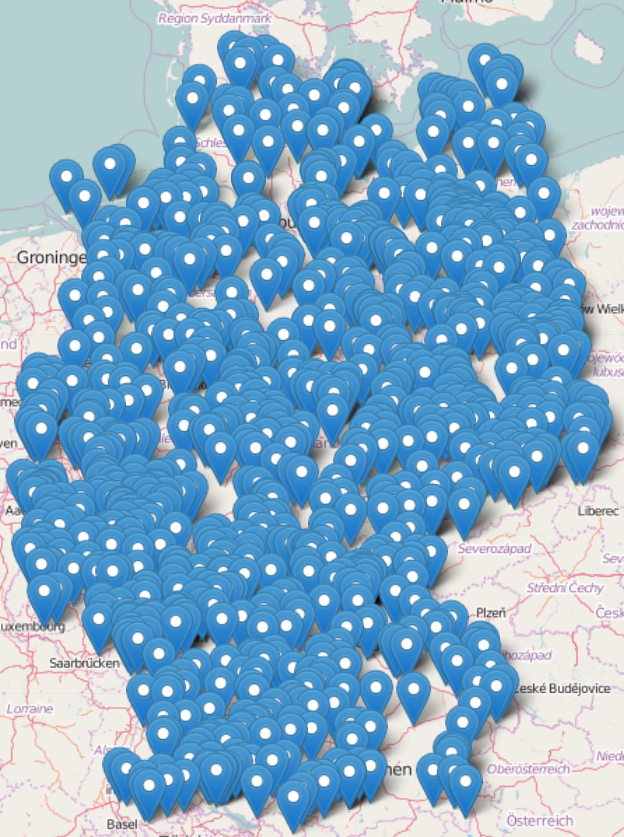
\includegraphics{figure/Germany_Campsites.PNG}

\end{frame}

\begin{frame}{Popups in einer interactiven Karte}

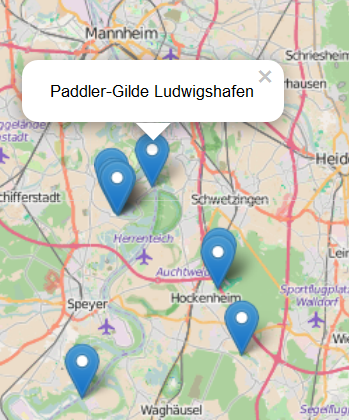
\includegraphics{figure/Camping_Mannheim.PNG}

Ich hab die Ergebnisse hochgeladen:

\url{http://rpubs.com/Japhilko82/Campsites}

\end{frame}

\begin{frame}{Wie man auf Rpubs publizieren kann}

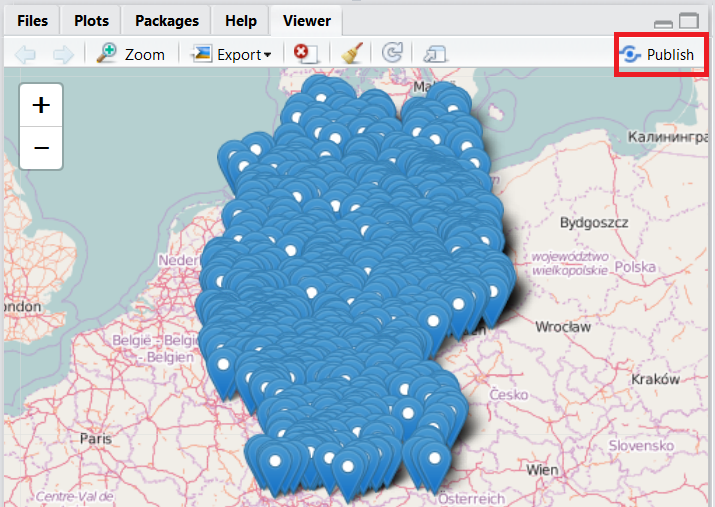
\includegraphics{figure/PublishCampSitesGermany.PNG}

\end{frame}

\begin{frame}[fragile]{Ein weiteres Beispiel - Weltkulturerbe}

\begin{Shaded}
\begin{Highlighting}[]
\NormalTok{url <-}\StringTok{ "https://raw.githubusercontent.com/Japhilko/}
\StringTok{GeoData/master/2015/data/whcSites.csv"}

\NormalTok{whcSites <-}\StringTok{ }\KeywordTok{read.csv}\NormalTok{(url) }
\end{Highlighting}
\end{Shaded}

\end{frame}

\begin{frame}[fragile]{Eine interaktive Karte erstellen}

\begin{Shaded}
\begin{Highlighting}[]
\NormalTok{m <-}\StringTok{ }\KeywordTok{leaflet}\NormalTok{() }\OperatorTok
\StringTok{  }\KeywordTok{addTiles}\NormalTok{() }\OperatorTok\StringTok{  }\CommentTok{# Add default OpenStreetMap map tiles}
\StringTok{  }\KeywordTok{addMarkers}\NormalTok{(}\DataTypeTok{lng=}\NormalTok{whcSites}\OperatorTok{$}\NormalTok{lon, }
             \DataTypeTok{lat=}\NormalTok{whcSites}\OperatorTok{$}\NormalTok{lat, }
             \DataTypeTok{popup=}\NormalTok{whcSites}\OperatorTok{$}\NormalTok{name_en)}
\NormalTok{m}
\end{Highlighting}
\end{Shaded}

\end{frame}

\begin{frame}{Die Karte zeigen}

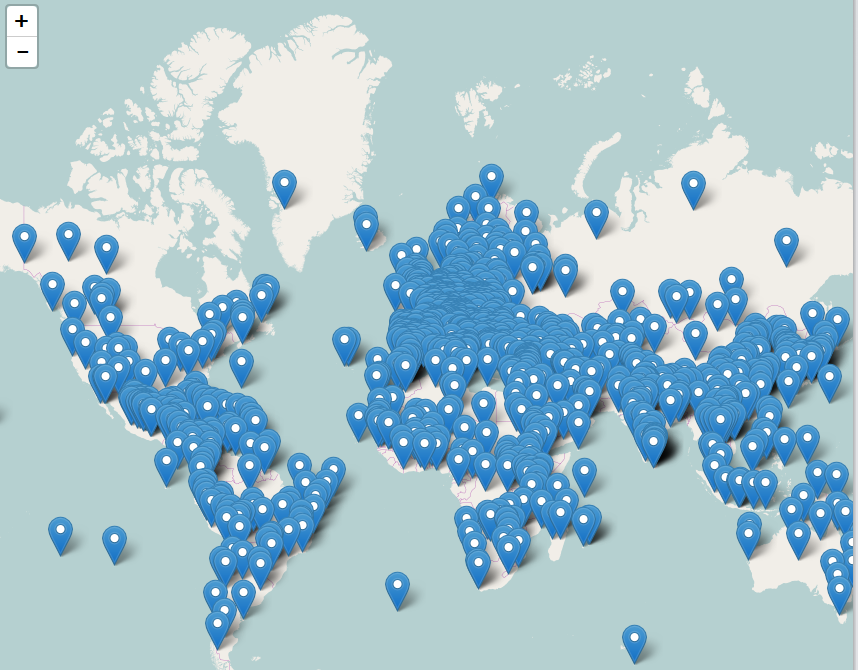
\includegraphics{figure/WHCPopUps.PNG}

\end{frame}

\begin{frame}[fragile]{Farbe hinzu}

\begin{Shaded}
\begin{Highlighting}[]
\NormalTok{whcSites}\OperatorTok{$}\NormalTok{color <-}\StringTok{ "red"}
\NormalTok{whcSites}\OperatorTok{$}\NormalTok{color[whcSites}\OperatorTok{$}\NormalTok{category}\OperatorTok{==}\StringTok{"Cultural"}\NormalTok{] <-}\StringTok{ "blue"}
\NormalTok{whcSites}\OperatorTok{$}\NormalTok{color[whcSites}\OperatorTok{$}\NormalTok{category}\OperatorTok{==}\StringTok{"Mixed"}\NormalTok{] <-}\StringTok{ "orange"}
\end{Highlighting}
\end{Shaded}

\end{frame}

\begin{frame}[fragile]{Eine Karte mit Farbe erzeugen}

\begin{Shaded}
\begin{Highlighting}[]
\NormalTok{m1 <-}\StringTok{ }\KeywordTok{leaflet}\NormalTok{() }\OperatorTok
\StringTok{  }\KeywordTok{addTiles}\NormalTok{() }\OperatorTok\StringTok{  }
\StringTok{  }\KeywordTok{addCircles}\NormalTok{(}\DataTypeTok{lng=}\NormalTok{whcSites}\OperatorTok{$}\NormalTok{lon, }
             \DataTypeTok{lat=}\NormalTok{whcSites}\OperatorTok{$}\NormalTok{lat, }
             \DataTypeTok{popup=}\NormalTok{whcSites}\OperatorTok{$}\NormalTok{name_en,}
             \DataTypeTok{color=}\NormalTok{whcSites}\OperatorTok{$}\NormalTok{color)}
\NormalTok{m1}
\end{Highlighting}
\end{Shaded}

\end{frame}

\begin{frame}{Die Karte zeigen}

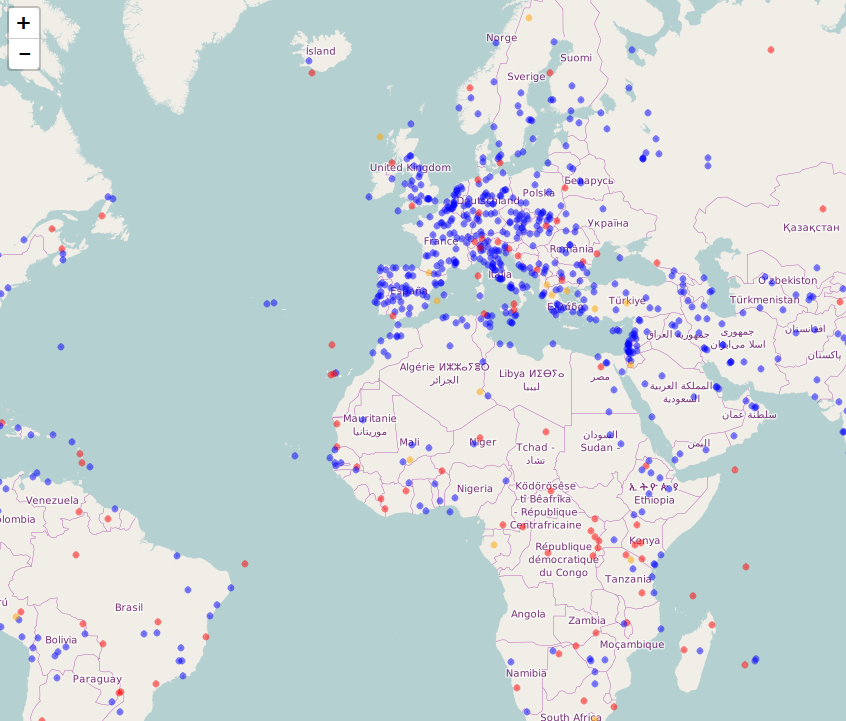
\includegraphics{figure/WHCcircles.PNG}

\end{frame}

\begin{frame}{\href{http://www.r-bloggers.com/interactive-mapping-with-leaflet-in-r-2/}{Die
Karte abspeichern}}

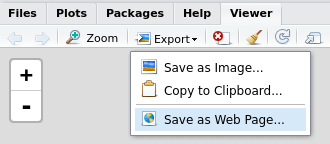
\includegraphics{figure/snapshot2.png}

\end{frame}

\begin{frame}[fragile]{Das Paket \texttt{mapview} - Beispieldatensatz
Franken}

\begin{Shaded}
\begin{Highlighting}[]
\KeywordTok{library}\NormalTok{(mapview)}

\KeywordTok{mapview}\NormalTok{(franconia)}
\end{Highlighting}
\end{Shaded}

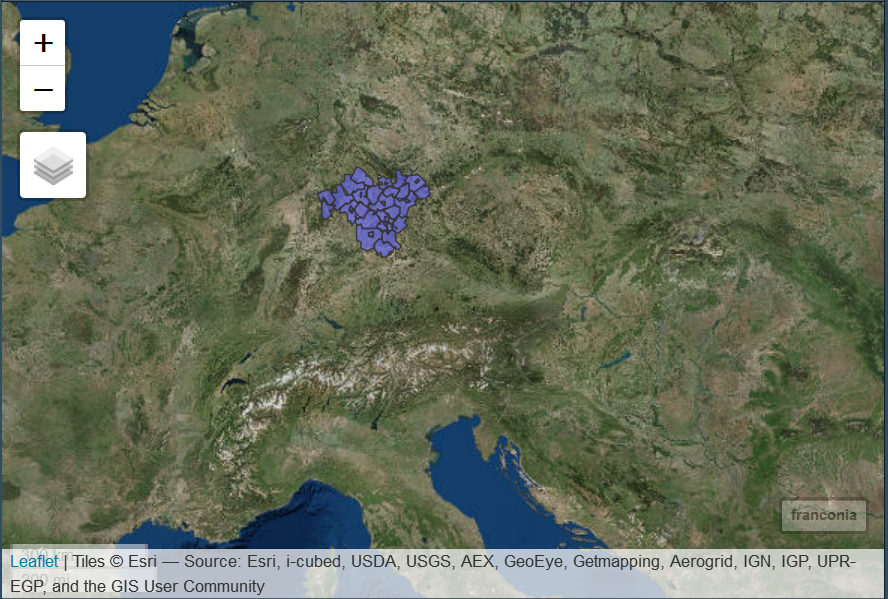
\includegraphics{figure/franconia.PNG}

\end{frame}

\begin{frame}[fragile]{GADM und \texttt{mapview}}

\begin{Shaded}
\begin{Highlighting}[]
\KeywordTok{mapview}\NormalTok{(leaflet}\OperatorTok{::}\NormalTok{gadmCHE)}
\end{Highlighting}
\end{Shaded}

\end{frame}

\begin{frame}[fragile]{Das Paket \texttt{mapview}}

\begin{Shaded}
\begin{Highlighting}[]
\KeywordTok{library}\NormalTok{(mapedit)}
\KeywordTok{library}\NormalTok{(magrittr)}

\NormalTok{lf <-}\StringTok{ }\KeywordTok{mapview}\NormalTok{()}
\NormalTok{drawing <-}\StringTok{ }\NormalTok{lf }\OperatorTok
\StringTok{  }\KeywordTok{editMap}\NormalTok{()}
\end{Highlighting}
\end{Shaded}

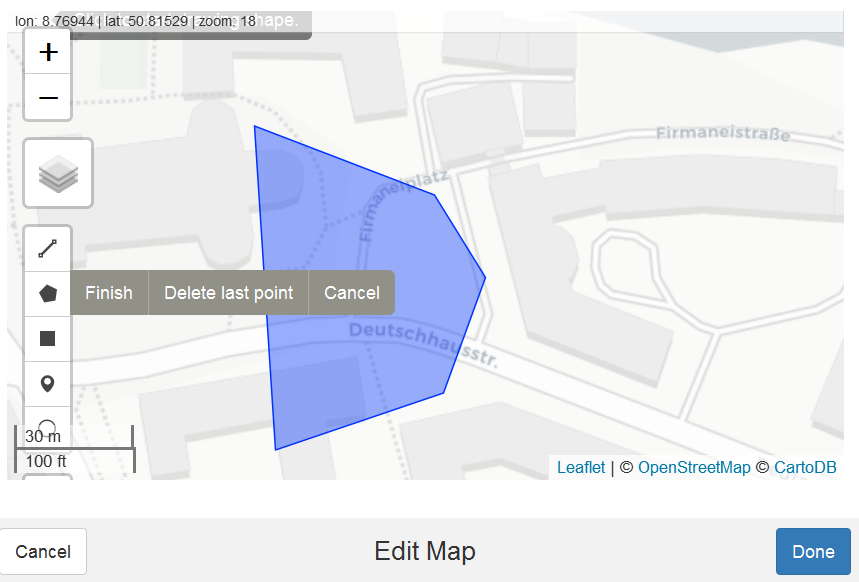
\includegraphics{figure/editmap.PNG}

\end{frame}

\begin{frame}[fragile]{Das Paket \texttt{mapview}}

\begin{Shaded}
\begin{Highlighting}[]
\KeywordTok{load}\NormalTok{(}\StringTok{"../data/spatsamp_68239.RData"}\NormalTok{)}
\end{Highlighting}
\end{Shaded}

\begin{Shaded}
\begin{Highlighting}[]
\KeywordTok{library}\NormalTok{(mapview)}
\KeywordTok{mapview}\NormalTok{(spatsamp)}
\end{Highlighting}
\end{Shaded}

\end{frame}

\begin{frame}[fragile]{Das Paket \texttt{leaflet}}

\begin{Shaded}
\begin{Highlighting}[]
\KeywordTok{library}\NormalTok{(}\StringTok{"tmaptools"}\NormalTok{)}
\NormalTok{gc_tma <-}\StringTok{ }\KeywordTok{geocode_OSM}\NormalTok{(}\StringTok{"Mannheim, GESIS"}\NormalTok{)}
\end{Highlighting}
\end{Shaded}

\begin{Shaded}
\begin{Highlighting}[]
\KeywordTok{library}\NormalTok{(leaflet)}
\KeywordTok{library}\NormalTok{(magrittr)}
\NormalTok{m <-}\StringTok{ }\KeywordTok{leaflet}\NormalTok{() }\OperatorTok
\KeywordTok{addTiles}\NormalTok{() }\OperatorTok
\KeywordTok{addMarkers}\NormalTok{(}\DataTypeTok{lng=}\FloatTok{8.463061}\NormalTok{ , }\DataTypeTok{lat=}\FloatTok{49.485736}\NormalTok{ , }\DataTypeTok{popup=}\StringTok{"GESIS Mannheim"}\NormalTok{)}
\NormalTok{m}
\end{Highlighting}
\end{Shaded}

\end{frame}

\begin{frame}[fragile]{Das Paket \texttt{geojsonR}}

\begin{itemize}
\tightlist
\item
  JavaScript Object Notation
\end{itemize}

\begin{Shaded}
\begin{Highlighting}[]
\KeywordTok{install.packages}\NormalTok{(}\StringTok{"geojsonR"}\NormalTok{)}
\KeywordTok{citation}\NormalTok{(}\StringTok{"geojsonR"}\NormalTok{)}
\end{Highlighting}
\end{Shaded}

\end{frame}

\begin{frame}[fragile]{Wo bekomme ich ein geojson}

\begin{itemize}
\tightlist
\item
  Ein
  \href{https://wiki.openstreetmap.org/wiki/Map_Features}{\textbf{OSM
  map feature}} heraus suchen
\item
  z.B. \texttt{key=highway}, \texttt{value=bus\_stop}
\item
  Auf \href{https://overpass-turbo.eu/}{\textbf{Overpass Turbo}} gehen
  und das Objekt herunterladen
\end{itemize}

\begin{Shaded}
\begin{Highlighting}[]
\NormalTok{bus_stops <-}\StringTok{ }\NormalTok{geojsonio}\OperatorTok{::}\KeywordTok{geojson_read}\NormalTok{(}\StringTok{"../data/Amsterdam_bus_stop.geojson"}\NormalTok{,}
  \DataTypeTok{what =} \StringTok{"sp"}\NormalTok{)}
\end{Highlighting}
\end{Shaded}

\end{frame}

\begin{frame}[fragile]{Die Punkte plotten}

\begin{Shaded}
\begin{Highlighting}[]
\NormalTok{sp}\OperatorTok{::}\KeywordTok{plot}\NormalTok{(bus_stops)}
\end{Highlighting}
\end{Shaded}


\includegraphics{slides_all2gether_part2_files/figure-beamer/unnamed-chunk-168-1.pdf}

\end{frame}

\begin{frame}[fragile]{\href{https://cran.r-project.org/web/packages/lawn/index.html}{Das
Paket \texttt{lawn}}}

\begin{itemize}
\item
  \href{https://cran.r-project.org/web/packages/lawn/vignettes/lawn_vignette.html}{\textbf{Vignette}}
  für das Paket \texttt{lawn}
\item
  Mit dem Paket \texttt{lawn} kann die Javascript-Bibliothek turf.js in
  R eingebunden werden.
\item
  Weitere genutzte Javascript Bibliotheken (geojson-random und
  geojsonhint), werden verwendet um GeoJSON-Objekte zufällig zu erzeugen
  bzw. um die GeoJSON Objekte einzufärben.
\end{itemize}

\begin{Shaded}
\begin{Highlighting}[]
\KeywordTok{install.packages}\NormalTok{(}\StringTok{"lawn"}\NormalTok{)}
\KeywordTok{citation}\NormalTok{(}\StringTok{"lawn"}\NormalTok{)}
\end{Highlighting}
\end{Shaded}

\begin{Shaded}
\begin{Highlighting}[]
\KeywordTok{library}\NormalTok{(lawn)}
\end{Highlighting}
\end{Shaded}

\end{frame}

\begin{frame}[fragile]{Ein zufälliges Beispiel Objekt erstellen}

\begin{itemize}
\tightlist
\item
  Mit der Funktion \texttt{gr\_polygon} kann ein Beispielobjekt erzeugt
  werden.
\item
  Anschließend kann man sich das Objekt mit der generischen Funktion
  \texttt{view} plotten.
\end{itemize}

\begin{Shaded}
\begin{Highlighting}[]
\NormalTok{a <-}\StringTok{ }\KeywordTok{gr_polygon}\NormalTok{(}\DataTypeTok{n =} \DecValTok{1}\NormalTok{, }\DataTypeTok{vertices =} \DecValTok{5}\NormalTok{, }\DataTypeTok{max_radial_length =} \DecValTok{5}\NormalTok{)}
\KeywordTok{view}\NormalTok{(a)}
\end{Highlighting}
\end{Shaded}

\begin{Shaded}
\begin{Highlighting}[]
\NormalTok{b <-}\StringTok{ }\KeywordTok{gr_polygon}\NormalTok{(}\DataTypeTok{n =} \DecValTok{1}\NormalTok{)}
\KeywordTok{view}\NormalTok{(b)}
\end{Highlighting}
\end{Shaded}

\end{frame}

\begin{frame}[fragile]{Interaktive Deutschland Karte}

\begin{Shaded}
\begin{Highlighting}[]
\NormalTok{gcs <-}\StringTok{ }\NormalTok{geojsonio}\OperatorTok{::}\KeywordTok{geojson_read}\NormalTok{(}\StringTok{"../data/ddat.geojson"}\NormalTok{)}
\KeywordTok{view}\NormalTok{(gcs)}
\end{Highlighting}
\end{Shaded}

\end{frame}

\begin{frame}[fragile]{Das Paket \texttt{jsonlite}}

\begin{itemize}
\tightlist
\item
  A Robust, High Performance JSON Parser and Generator for R
\end{itemize}

\begin{Shaded}
\begin{Highlighting}[]
\KeywordTok{library}\NormalTok{(jsonlite)}
\NormalTok{geoc <-}\StringTok{ }\KeywordTok{read_json}\NormalTok{(}\StringTok{"../data/ddat.geojson"}\NormalTok{)}
\end{Highlighting}
\end{Shaded}

\begin{Shaded}
\begin{Highlighting}[]
\KeywordTok{citation}\NormalTok{(}\StringTok{"jsonlite"}\NormalTok{)}
\end{Highlighting}
\end{Shaded}

\begin{verbatim}
## 
## To cite jsonlite in publications use:
## 
##   Jeroen Ooms (2014). The jsonlite Package: A Practical and
##   Consistent Mapping Between JSON Data and R Objects.
##   arXiv:1403.2805 [stat.CO] URL https://arxiv.org/abs/1403.2805.
## 
## A BibTeX entry for LaTeX users is
## 
##   @Article{,
##     title = {The jsonlite Package: A Practical and Consistent Mapping Between JSON Data and R Objects},
##     author = {Jeroen Ooms},
##     journal = {arXiv:1403.2805 [stat.CO]},
##     year = {2014},
##     url = {https://arxiv.org/abs/1403.2805},
##   }
\end{verbatim}

\end{frame}

\begin{frame}[fragile]{Das Paket \texttt{RJSONIO}}

\begin{Shaded}
\begin{Highlighting}[]
\KeywordTok{library}\NormalTok{(}\StringTok{"RJSONIO"}\NormalTok{)}
\NormalTok{con <-}\StringTok{ }\KeywordTok{url}\NormalTok{(}\StringTok{"http://nominatim.openstreetmap.org/search?format=json&}
\StringTok{addressdetails=1&extratags=1&q=Amsterdam+Niederlande+Rozengracht+1"}\NormalTok{)}
\NormalTok{geoc <-}\StringTok{ }\KeywordTok{fromJSON}\NormalTok{(}\KeywordTok{paste}\NormalTok{(}\KeywordTok{readLines}\NormalTok{(con,}\DataTypeTok{warn=}\NormalTok{F), }
                       \DataTypeTok{collapse =} \StringTok{''}\NormalTok{))}
\KeywordTok{close}\NormalTok{(con)}
\end{Highlighting}
\end{Shaded}

\end{frame}

\begin{frame}{Links und Quellen}

\begin{itemize}
\item
  \href{http://www.r-bloggers.com/the-leaflet-package-for-online-mapping-in-r/}{Rbloggers
  Artikel zu Leaflet}
\item
  \href{https://rstudio.github.io/leaflet/}{Einführung in Leaflet für R}
\item
  \href{https://blog.hwr-berlin.de/codeandstats/category/scientific-software/r/}{Offline
  Karten mit RgoogleMaps und leaflet}
\item
  \href{https://github.com/ropensci/lawn}{github Ordner für das lwan
  Paket}
\end{itemize}

\end{frame}

\begin{frame}[fragile]{Themen dieses Abschnitts}

\begin{itemize}
\tightlist
\item
  Der Import von Geodaten mit dem Paket simple features (\texttt{sf}).
\item
  Die Verarbeitung der OSM-Daten mit dem Paket \texttt{sf}.
\item
  Die Daten visualisieren mit \texttt{sf}
\end{itemize}

\end{frame}

\begin{frame}[fragile]{Das Paket \texttt{sf}}

\begin{quote}
Simple Features for R
\end{quote}

\begin{Shaded}
\begin{Highlighting}[]
\KeywordTok{library}\NormalTok{(sf)}
\end{Highlighting}
\end{Shaded}

\begin{itemize}
\tightlist
\item
  Ein Demo ist im Paket \texttt{sf} integriert
\end{itemize}

\begin{Shaded}
\begin{Highlighting}[]
\KeywordTok{demo}\NormalTok{(sf}\OperatorTok{::}\NormalTok{affine)}
\end{Highlighting}
\end{Shaded}


\includegraphics{figure/Rplot.pdf}

\end{frame}

\begin{frame}[fragile]{Beispieldaten bekommen}

\begin{Shaded}
\begin{Highlighting}[]
\KeywordTok{library}\NormalTok{(osmdata)}
\NormalTok{bb_poly <-}\StringTok{ }\KeywordTok{getbb}\NormalTok{(}\DataTypeTok{place_name =} \StringTok{"Amsterdam"}\NormalTok{, }
                 \DataTypeTok{format_out =} \StringTok{"polygon"}\NormalTok{)}
\end{Highlighting}
\end{Shaded}

\begin{Shaded}
\begin{Highlighting}[]
\NormalTok{ls <-}\StringTok{ }\KeywordTok{st_multilinestring}\NormalTok{(bb_poly)}
\end{Highlighting}
\end{Shaded}

\begin{Shaded}
\begin{Highlighting}[]
\NormalTok{pol <-}\StringTok{ }\NormalTok{sf}\OperatorTok{::}\KeywordTok{st_polygon}\NormalTok{(bb_poly)}
\KeywordTok{class}\NormalTok{(pol)}
\end{Highlighting}
\end{Shaded}

\begin{verbatim}
## [1] "XY"      "POLYGON" "sfg"
\end{verbatim}

\begin{Shaded}
\begin{Highlighting}[]
\NormalTok{bb_poly_ma <-}\StringTok{ }\KeywordTok{getbb}\NormalTok{(}\DataTypeTok{place_name =} \StringTok{"Mannheim"}\NormalTok{, }
                 \DataTypeTok{format_out =} \StringTok{"polygon"}\NormalTok{)}
\end{Highlighting}
\end{Shaded}

\end{frame}

\begin{frame}[fragile]{Das Ergebnis plotten}

\begin{Shaded}
\begin{Highlighting}[]
\KeywordTok{plot}\NormalTok{(bb_poly_ma)}
\end{Highlighting}
\end{Shaded}

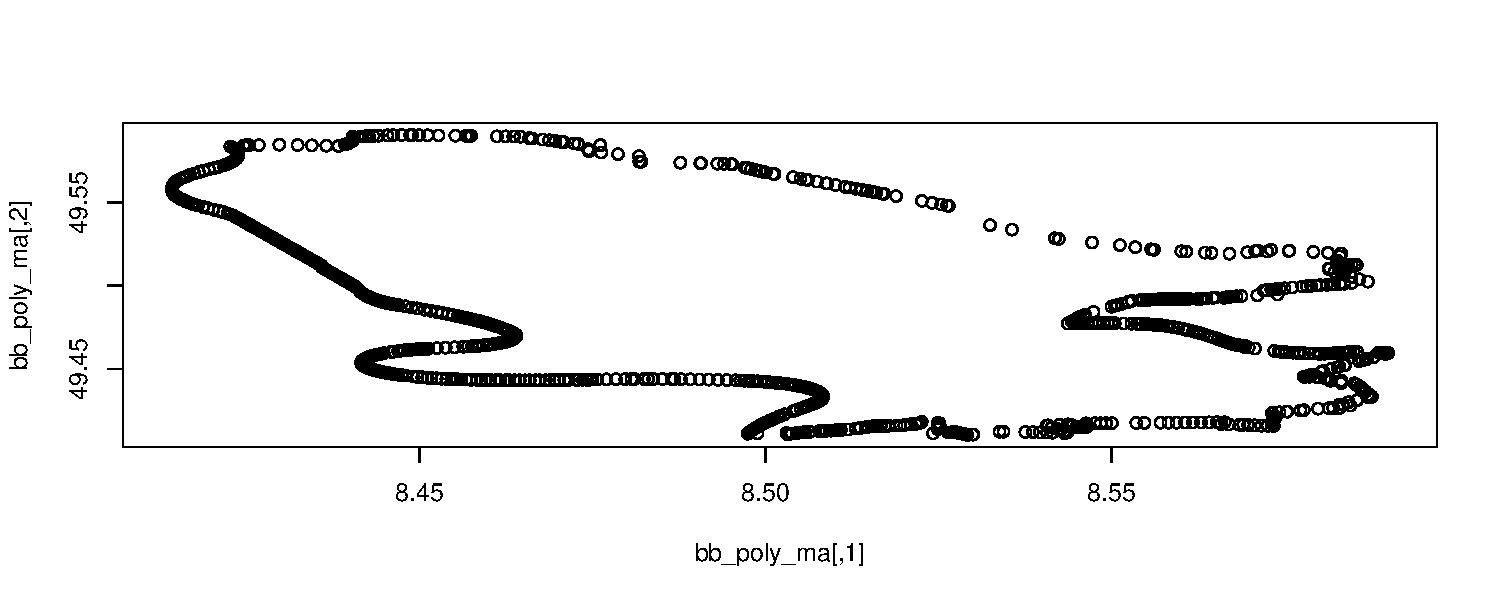
\includegraphics{slides_all2gether_part2_files/figure-beamer/unnamed-chunk-185-1.pdf}

\end{frame}

\begin{frame}[fragile]{Ein Beispieldatensatz}

\begin{Shaded}
\begin{Highlighting}[]
\KeywordTok{demo}\NormalTok{(nc, }\DataTypeTok{ask =} \OtherTok{FALSE}\NormalTok{, }\DataTypeTok{echo =} \OtherTok{FALSE}\NormalTok{)}
\end{Highlighting}
\end{Shaded}

\begin{verbatim}
## Reading layer `nc.gpkg' from data source `D:\Programme\R-3.5.0\library\sf\gpkg\nc.gpkg' using driver `GPKG'
## Simple feature collection with 100 features and 14 fields
## Attribute-geometry relationship: 0 constant, 8 aggregate, 6 identity
## geometry type:  MULTIPOLYGON
## dimension:      XY
## bbox:           xmin: -84.32385 ymin: 33.88199 xmax: -75.45698 ymax: 36.58965
## epsg (SRID):    4267
## proj4string:    +proj=longlat +datum=NAD27 +no_defs
\end{verbatim}

\end{frame}

\begin{frame}[fragile]{\href{https://r-spatial.github.io/sf/articles/sf5.html}{Graphiken
mit \texttt{sf}}}

\begin{Shaded}
\begin{Highlighting}[]
\KeywordTok{plot}\NormalTok{(nc)}
\end{Highlighting}
\end{Shaded}

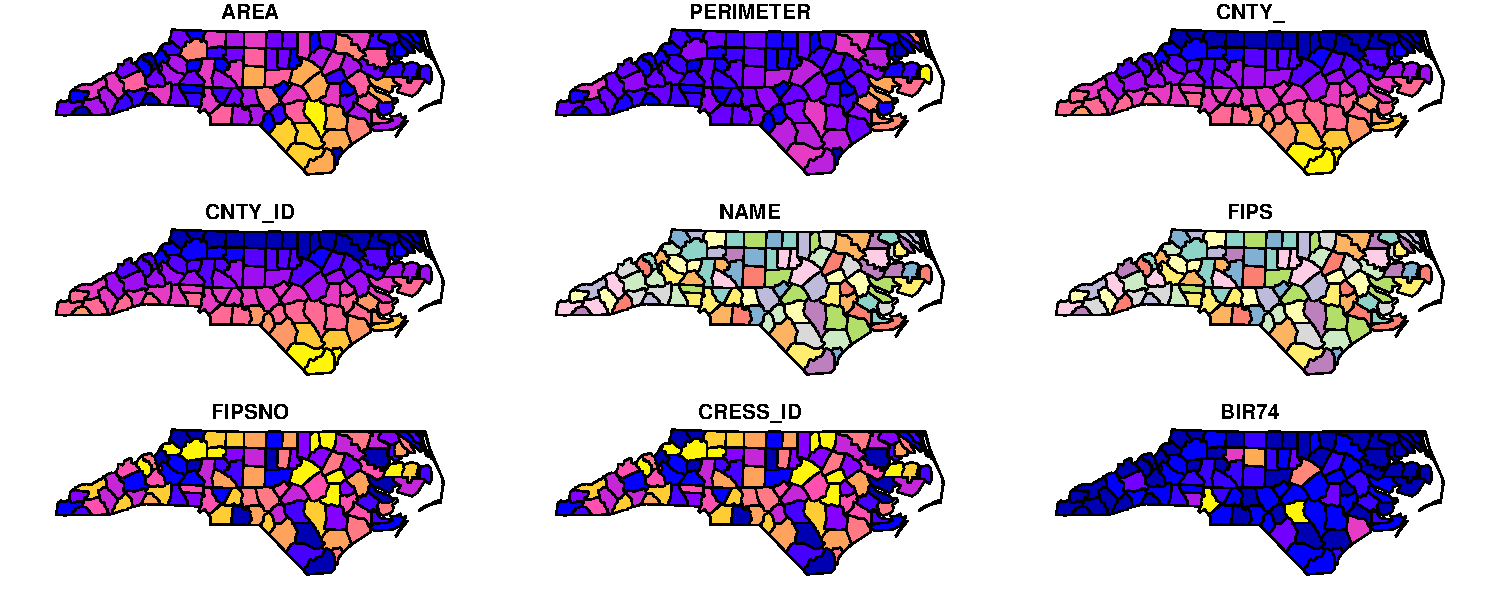
\includegraphics{slides_all2gether_part2_files/figure-beamer/unnamed-chunk-191-1.pdf}

\end{frame}

\begin{frame}[fragile]{\href{https://cran.r-project.org/web/packages/sf/vignettes/sf2.html}{Shapefiles
mit \texttt{sf} importieren}}

\begin{Shaded}
\begin{Highlighting}[]
\NormalTok{lon <-}\StringTok{ }\KeywordTok{st_read}\NormalTok{(}\StringTok{"../data/london_sport.shp"}\NormalTok{)}
\end{Highlighting}
\end{Shaded}

\begin{verbatim}
## Reading layer `london_sport' from data source `D:\Daten\GitHub\geocourse\data\london_sport.shp' using driver `ESRI Shapefile'
## Simple feature collection with 33 features and 4 fields
## geometry type:  POLYGON
## dimension:      XY
## bbox:           xmin: 503571.2 ymin: 155850.8 xmax: 561941.1 ymax: 200932.5
## epsg (SRID):    NA
## proj4string:    +proj=tmerc +lat_0=49 +lon_0=-2 +k=0.9996012717 +x_0=400000 +y_0=-100000 +ellps=airy +units=m +no_defs
\end{verbatim}

\end{frame}

\begin{frame}[fragile]{Das Shapefile plotten}

\begin{Shaded}
\begin{Highlighting}[]
\KeywordTok{plot}\NormalTok{(lon}\OperatorTok{$}\NormalTok{geometry)}
\end{Highlighting}
\end{Shaded}


\includegraphics{slides_all2gether_part2_files/figure-beamer/unnamed-chunk-195-1.pdf}

\end{frame}

\begin{frame}[fragile]{Daten vom Amsterdam Beispiel}

\begin{Shaded}
\begin{Highlighting}[]
\NormalTok{datm <-}\StringTok{ }\KeywordTok{st_read}\NormalTok{(}\StringTok{"../data/ams_centraal.osm"}\NormalTok{,}\StringTok{"multipolygons"}\NormalTok{)}
\end{Highlighting}
\end{Shaded}

\begin{verbatim}
## Reading layer `multipolygons' from data source `D:\Daten\GitHub\geocourse\data\ams_centraal.osm' using driver `OSM'
## Simple feature collection with 2796 features and 25 fields
## geometry type:  MULTIPOLYGON
## dimension:      XY
## bbox:           xmin: 4.874776 ymin: 52.36088 xmax: 4.929755 ymax: 52.39393
## epsg (SRID):    4326
## proj4string:    +proj=longlat +datum=WGS84 +no_defs
\end{verbatim}

\end{frame}

\begin{frame}[fragile]{\href{https://cran.r-project.org/web/packages/sf/vignettes/sf3.html}{Die
Funktion \texttt{st\_geometry}}}

\begin{Shaded}
\begin{Highlighting}[]
\NormalTok{geom_datm <-}\StringTok{ }\KeywordTok{st_geometry}\NormalTok{(datm)}
\KeywordTok{plot}\NormalTok{(geom_datm)}
\end{Highlighting}
\end{Shaded}


\includegraphics{slides_all2gether_part2_files/figure-beamer/unnamed-chunk-197-1.pdf}

\end{frame}

\begin{frame}[fragile]{Die Häuser auswählen}

\begin{Shaded}
\begin{Highlighting}[]
\KeywordTok{library}\NormalTok{(dplyr)}
\NormalTok{buis <-}\StringTok{ }\NormalTok{datm }\OperatorTok\StringTok{ }\KeywordTok{select}\NormalTok{(building)}
\KeywordTok{plot}\NormalTok{(buis)}
\end{Highlighting}
\end{Shaded}

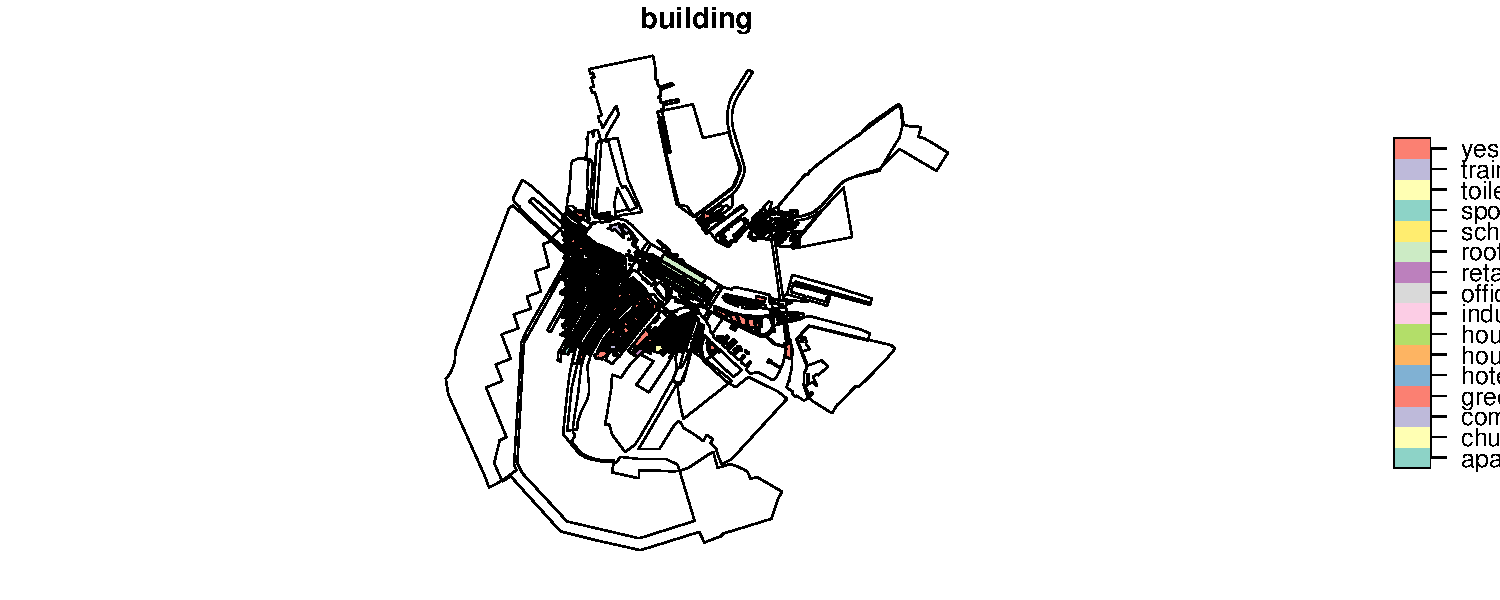
\includegraphics{slides_all2gether_part2_files/figure-beamer/unnamed-chunk-198-1.pdf}

\end{frame}

\begin{frame}[fragile]{Welche Häusertypen gibt es?}

\begin{Shaded}
\begin{Highlighting}[]
\NormalTok{buis2 <-}\StringTok{ }\NormalTok{datm }\OperatorTok\StringTok{ }\NormalTok{as.data.frame }\OperatorTok\StringTok{ }\KeywordTok{select}\NormalTok{(building)}
\end{Highlighting}
\end{Shaded}

\begin{Shaded}
\begin{Highlighting}[]
\NormalTok{datbuis <-}\StringTok{ }\NormalTok{datm[, }\StringTok{"building"}\NormalTok{, drop =}\StringTok{ }\OtherTok{TRUE}\NormalTok{]}
\KeywordTok{plot}\NormalTok{(datbuis)}
\end{Highlighting}
\end{Shaded}

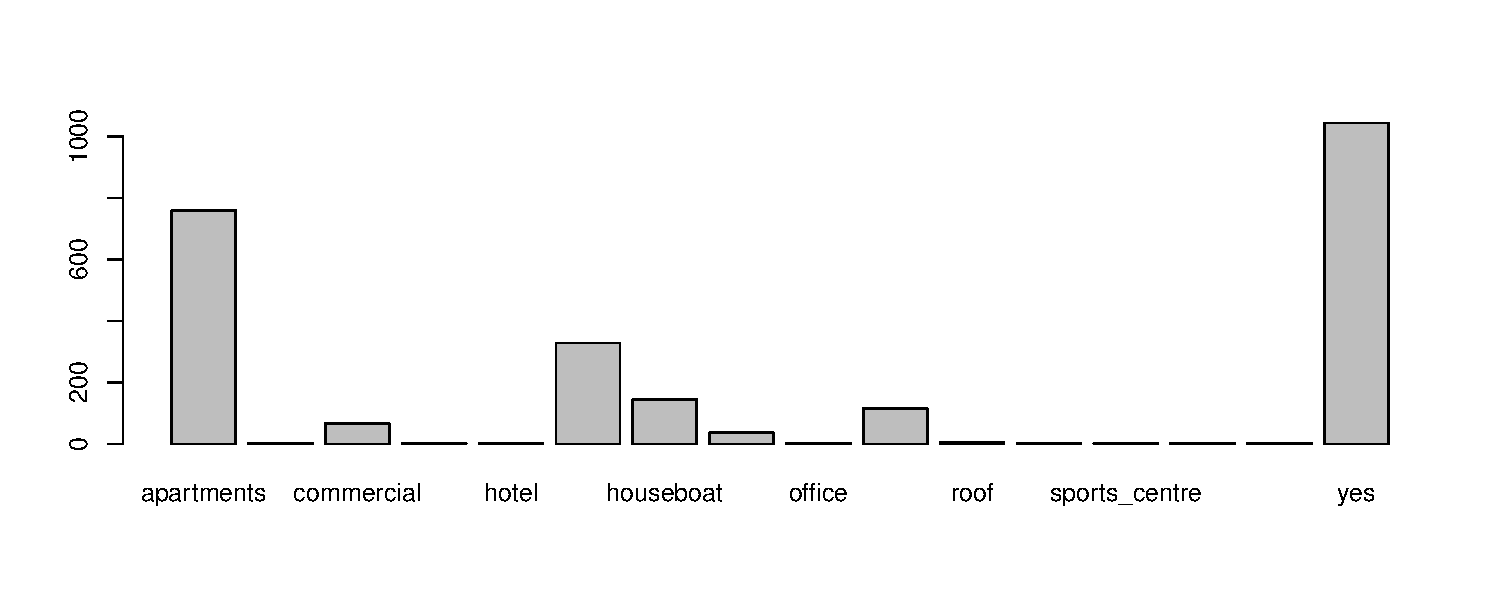
\includegraphics{slides_all2gether_part2_files/figure-beamer/unnamed-chunk-200-1.pdf}

\end{frame}

\begin{frame}[fragile]{}

\begin{Shaded}
\begin{Highlighting}[]
\NormalTok{houses <-}\StringTok{ }\NormalTok{datm[datm}\OperatorTok{$}\NormalTok{building }\OperatorTok{==}\StringTok{ "house"}\NormalTok{,]}
\KeywordTok{class}\NormalTok{(houses)}
\end{Highlighting}
\end{Shaded}

\begin{verbatim}
## [1] "sf"         "data.frame"
\end{verbatim}

\begin{Shaded}
\begin{Highlighting}[]
\NormalTok{## [1] "sf"         "data.frame"}
\NormalTok{dhous <-}\StringTok{ }\NormalTok{datm[houses,]}
\KeywordTok{plot}\NormalTok{(dhous}\OperatorTok{$}\NormalTok{geometry)}
\end{Highlighting}
\end{Shaded}


\includegraphics{slides_all2gether_part2_files/figure-beamer/unnamed-chunk-201-1.pdf}

\begin{Shaded}
\begin{Highlighting}[]
\KeywordTok{plot}\NormalTok{(}\KeywordTok{st_geometry}\NormalTok{(houses))}
\end{Highlighting}
\end{Shaded}


\includegraphics{slides_all2gether_part2_files/figure-beamer/unnamed-chunk-202-1.pdf}

\end{frame}

\begin{frame}[fragile]{\href{https://cran.r-project.org/web/packages/sf/vignettes/sf4.html}{Alle
Häuser herausnehmen}}

\begin{Shaded}
\begin{Highlighting}[]
\NormalTok{houses <-}\StringTok{ }\NormalTok{datm[datm}\OperatorTok{$}\NormalTok{building }\OperatorTok\StringTok{ }\KeywordTok{c}\NormalTok{(}\StringTok{"house"}\NormalTok{,}\StringTok{"yes"}\NormalTok{,}
                                    \StringTok{"apartments"}\NormalTok{),]}
\KeywordTok{plot}\NormalTok{(}\KeywordTok{st_geometry}\NormalTok{(houses))}
\end{Highlighting}
\end{Shaded}


\includegraphics{slides_all2gether_part2_files/figure-beamer/unnamed-chunk-203-1.pdf}

\end{frame}

\begin{frame}{Die Vignetten für das Paket \texttt{sf}}

\url{https://r-spatial.github.io/sf/reference/st_as_sf.html}

\url{https://r-spatial.github.io/sf/reference/st_read.html}

\url{https://r-spatial.github.io/sf/articles/sf1.html}

\end{frame}

\end{document}
